\documentclass[12pt]{article}
\usepackage{graphicx} % Required for inserting images
\usepackage{hyperref}
\usepackage{amsmath}
\usepackage{caption}
\usepackage{subcaption}
\usepackage{biblatex}
\usepackage{booktabs}
\usepackage{float}
\usepackage{threeparttable}

\addbibresource{citations.bib}
\usepackage[margin=1in]{geometry}
\usepackage{setspace}

\doublespacing

\begin{document}
%============Title page============

\begin{titlepage}
   \begin{center}
       \vspace*{1cm}

        \Large
        \textbf{Analysis of Ta-Re Alloys for Use in Superconducting Qubits}

        \vspace*{1cm}
        \normalsize
        \textbf{Daniel Jung}

        \vspace{0.5cm}
        Advised by Prof. Nathalie de Leon
            
       \vspace{1.5cm}
 
       \vfill
            
       Submitted in partial fulfillment of the requirements for the degree of Bachelor of Science in Engineering.
            
       \vspace{0.8cm}
            
       Department of Electrical and Computer Engineering\\
       Princeton University\\
       United States\\
       04/13/2026
            
   \end{center}
\end{titlepage}


\newpage

%============Original work============
\vspace{2cm}
\begin{center}
    I hereby declare that this Independent Work report represents my own work in accordance with University Regulations.\\
    \vspace{0.5cm}
    I hereby declare that this Independent Work report does not include regulated human subjects research.\\
    \vspace{0.5cm}
    I hereby declare that this Independent Work report does not include regulated animal subjects research.\\
    \vspace{0.5cm}
    /s/ Daniel Jung
\end{center}
\vfill

\newpage

%============Abstract============

\thispagestyle{plain}
\begin{center}
    \Large
    \textbf{Analysis of Ta-Re Alloys for Use in Superconducting Qubits}
        
    \vspace{0.4cm}
    \large
    \textbf{Daniel Jung}
       
    \vspace{0.9cm}
    \textbf{Abstract}
\normalsize
\end{center}
Superconducting qubits are among the leading platforms for quantum computing, where material choice critically impacts qubit coherence and scalability. Tantalum (Ta) has emerged as a promising candidate due to its stable, self-limiting oxide ($Ta_2O_5$), which hosts fewer dielectric two-level systems (TLS). Ta transmons on high-resist silicon exhibit lifetimes ($T_1$) up to 1.68 ms and Q factors up to $2.5 \times 10^7$ \cite{bland2025}. Rhenium (Re) also forms an exceptionally thin and inert oxide layer, and has demonstrated resonator quality factors exceeding $2\times 10^6$ \cite{crisa2025}. By alloying Ta with Re, we aim to combine Ta's low-loss coherence performance with Re's enhanced surface and structural properties. Ta--Re alloys may offer tailored superconducting behavior, improved oxidation resistance, and reduced TLS density---potentially surpassing pure Ta in coherence and fabrication resilience. This research explores the stability and oxidation behavior of thin-film Ta-Re alloys deposited on sapphire substrate.

\newpage

%============Abstract============

\tableofcontents

\newpage
%============Begin============

\thispagestyle{plain}

\section{Introduction}

\subsection{Superconducting Qubits and Decoherence}
Superconducting qubits are among the most promising platforms for realizing scalable quantum computers, offering fast gate times, lithographic scalability, and integrated microwave control. Implementations such as the transmon, fluxonium, and flux qubit leverage nonlinear Josephson junctions embedded in superconducting microwave circuits to store and manipulate quantum information. These devices rely on operation at ultra-low temperatures to maintain a superconductive state, minimizing energy loss and preserving quantum coherence.

While state-of-the-art superconducting qubits have achieved remarkable milestones---gate fidelities above 99.9\% and integration into multi-qubit processors with quantum error correction techniques \cite{marxer2025, acharya2025}---performance remains  limited by \textit{decoherence mechanisms} originating at materials interfaces. One of the dominant sources of decoherence is dielectric loss from two-level system (TLS) defects. Existing studies suggest two-level systems arise from structural disorder, trapped charges, and amorphous oxide layers at the substrate-metal, metal-air, and substrate-air interfaces, all of which absorb energy from the qubit's microwave field \cite{crowley2023, mclellan2023}. Advancing quantum coherence necessitates the discovery and engineering of new materials that exhibit chemically stable, low-loss surfaces and robust superconducting properties.

\subsection{Promising Platforms: Tantalum and Rhenium}
Recent research by Chang, Mclellan, et. al. suggests tantalum (Ta) may be a breakthrough platform for superconducting qubits. Tantalum's advantage lies in its native oxide layer, which forms a "relatively benign, self-limiting, and stoichiometric $Ta_2O_5$ film" \cite{mclellan2023}. This stable passivation reduces the density of amorphous TLS defects compared to traditional materials like niobium or aluminum. Devices fabricated from $\alpha$-phase Ta (bcc) on high-resistivity silicon substrates have enabled $T_1$ relaxation times reaching 1.68 ms and resonator quality factors ($Q$) up to $2.5 \times 10^7$ \cite{bland2025}.

Similar to Ta, rhenium (Re) has emerged also as a promising candidate for ultra-low-loss superconducting circuits. Re is distinguished by an extraordinarily thin and inert native oxide, which significantly curtails surface dielectric participation in microwave losses. Recent studies on Re-based microwave resonators have demonstrated high internal quality factors exceeding $2 \times 10^6$ \cite{crisa2025, ganjam2023}. Furthermore, transmon qubits leveraging Re as a base material have recently been established as a viable platform for long-lived coherence \cite{wang2026rhenium}. 

However, Re's utility in monolithic superconducting qubits is constrained by its low bulk critical temperature ($T_c \approx 1.7$--$2.0$\,K). Although the low $T_c$ is sufficient for basic cryogenic operation, it heightens sensitivity to thermal quasi-particle generation, limiting standalone deployment.

\subsection{Motivation for Tantalum-Rhenium Alloys}
To circumvent the limitations of pure Re and further optimize the favorable properties of Ta, material engineering through alloying presents a tempting strategy. Recent work has shown that alloying Ta with other transition metals, such as hafnium (Hf), can systematically tune the superconducting gap and increase $T_c$ while maintaining low-loss characteristics \cite{yang2026tantalum}. Similarly, tantalum-rhenium (Ta-Re) alloys offer a highly tunable parameter space aimed at combining the high $T_c$ and process compatibility of Ta with the ultra-thin oxide properties of Re \cite{mamiya1970superconductivity_ta_re}. Ta-Re thin films have further garnered interest in spintronics for their emergent spin Hall conductivity \cite{janus2025}, highlighting the rich interplay between their electronic and structural phases.

Of particular interest are Re-rich alloys. Although bulk Re has a low $T_c$, thin films with substantial Re content may exhibit significantly elevated critical temperatures driven by disorder and morphological modifications. For example, amorphous Re films have shown a $T_c \approx 7$--$8$\,K \cite{tarkaeva2025}, and electroplated Re in multilayers with noble metals achieves a $T_c$ up to 6\,K \cite{pappas2018}. An 80\% Re and 20\% Ta alloy composition seeks to exploit these disorder-induced enhancements in $T_c$ while retaining Re's promising surface chemistry. 

Because surface oxides are the primary host for TLS defects, understanding the exact chemical composition of the Ta-Re oxide interface is critical. Previous X-ray photoelectron spectroscopy (XPS) studies of Re have established its complex oxidation behavior, identifying multiple oxidation states ranging from metallic $Re^0$ to $Re^{7+}$ in $Re_2O_7$, which can vary drastically depending on the environment or the presence of secondary metals like platinum \cite{greiner2014, cimino1980photoelectron, tysoe1988xps}. However, the oxidation dynamics of Re when alloyed with a metal like Ta remain largely unexplored in the context of quantum circuit fabrication.

\subsection{Thesis Objectives}
The core objective of this thesis is to investigate the surface stability and oxidation behavior of an 80\% Re / 20\% Ta superconducting thin film to evaluate its viability for low-noise, high-coherence quantum circuits. Using time-resolved X-ray photoelectron spectroscopy (XPS), this systematically profiles the oxide growth and chemical speciation of the Ta-Re alloy following a buffered oxide etch (BOE). By dissecting the resulting surface stoichiometry, this work aims to identify potential sources of TLS dielectric loss and provide insights into engineering optimized Ta-Re interfaces for use in superconducting qubits.

\newpage

\section{Experiment}
\subsection{Preparation and Measurement}
All experiments were done using a previously fabricated 80\% Re 20\% Ta film deposited on sapphire substrate through co-sputtering. In order to monitor oxide growth, samples were first treated for 20 minutes in 10:1 buffered oxide etch (BOE) solution to etch away most native oxide. While an initial cleanse in piranha solution (H$_{2}$SO$_{4}$:H$_{2}$O$_{2}$) was attempted in order to ensure a clean surface, the film on one sample was quickly etched off (see Figure \ref{fig:piranha_etch}). Pure tantalum is known to survive piranha cleaning while pure rhenium does not\cite{wang2026rhenium}. One motivation for alloying Ta and Re was to leverage the process compatibility of Ta; however, this result visually demonstrates that a rhenium-rich alloy does not necessarily inherit Ta's chemical robustness to aggressive oxidation, remaining highly susceptible to standard semiconductor acid treatments. 

\begin{figure}[H]
    \centering
    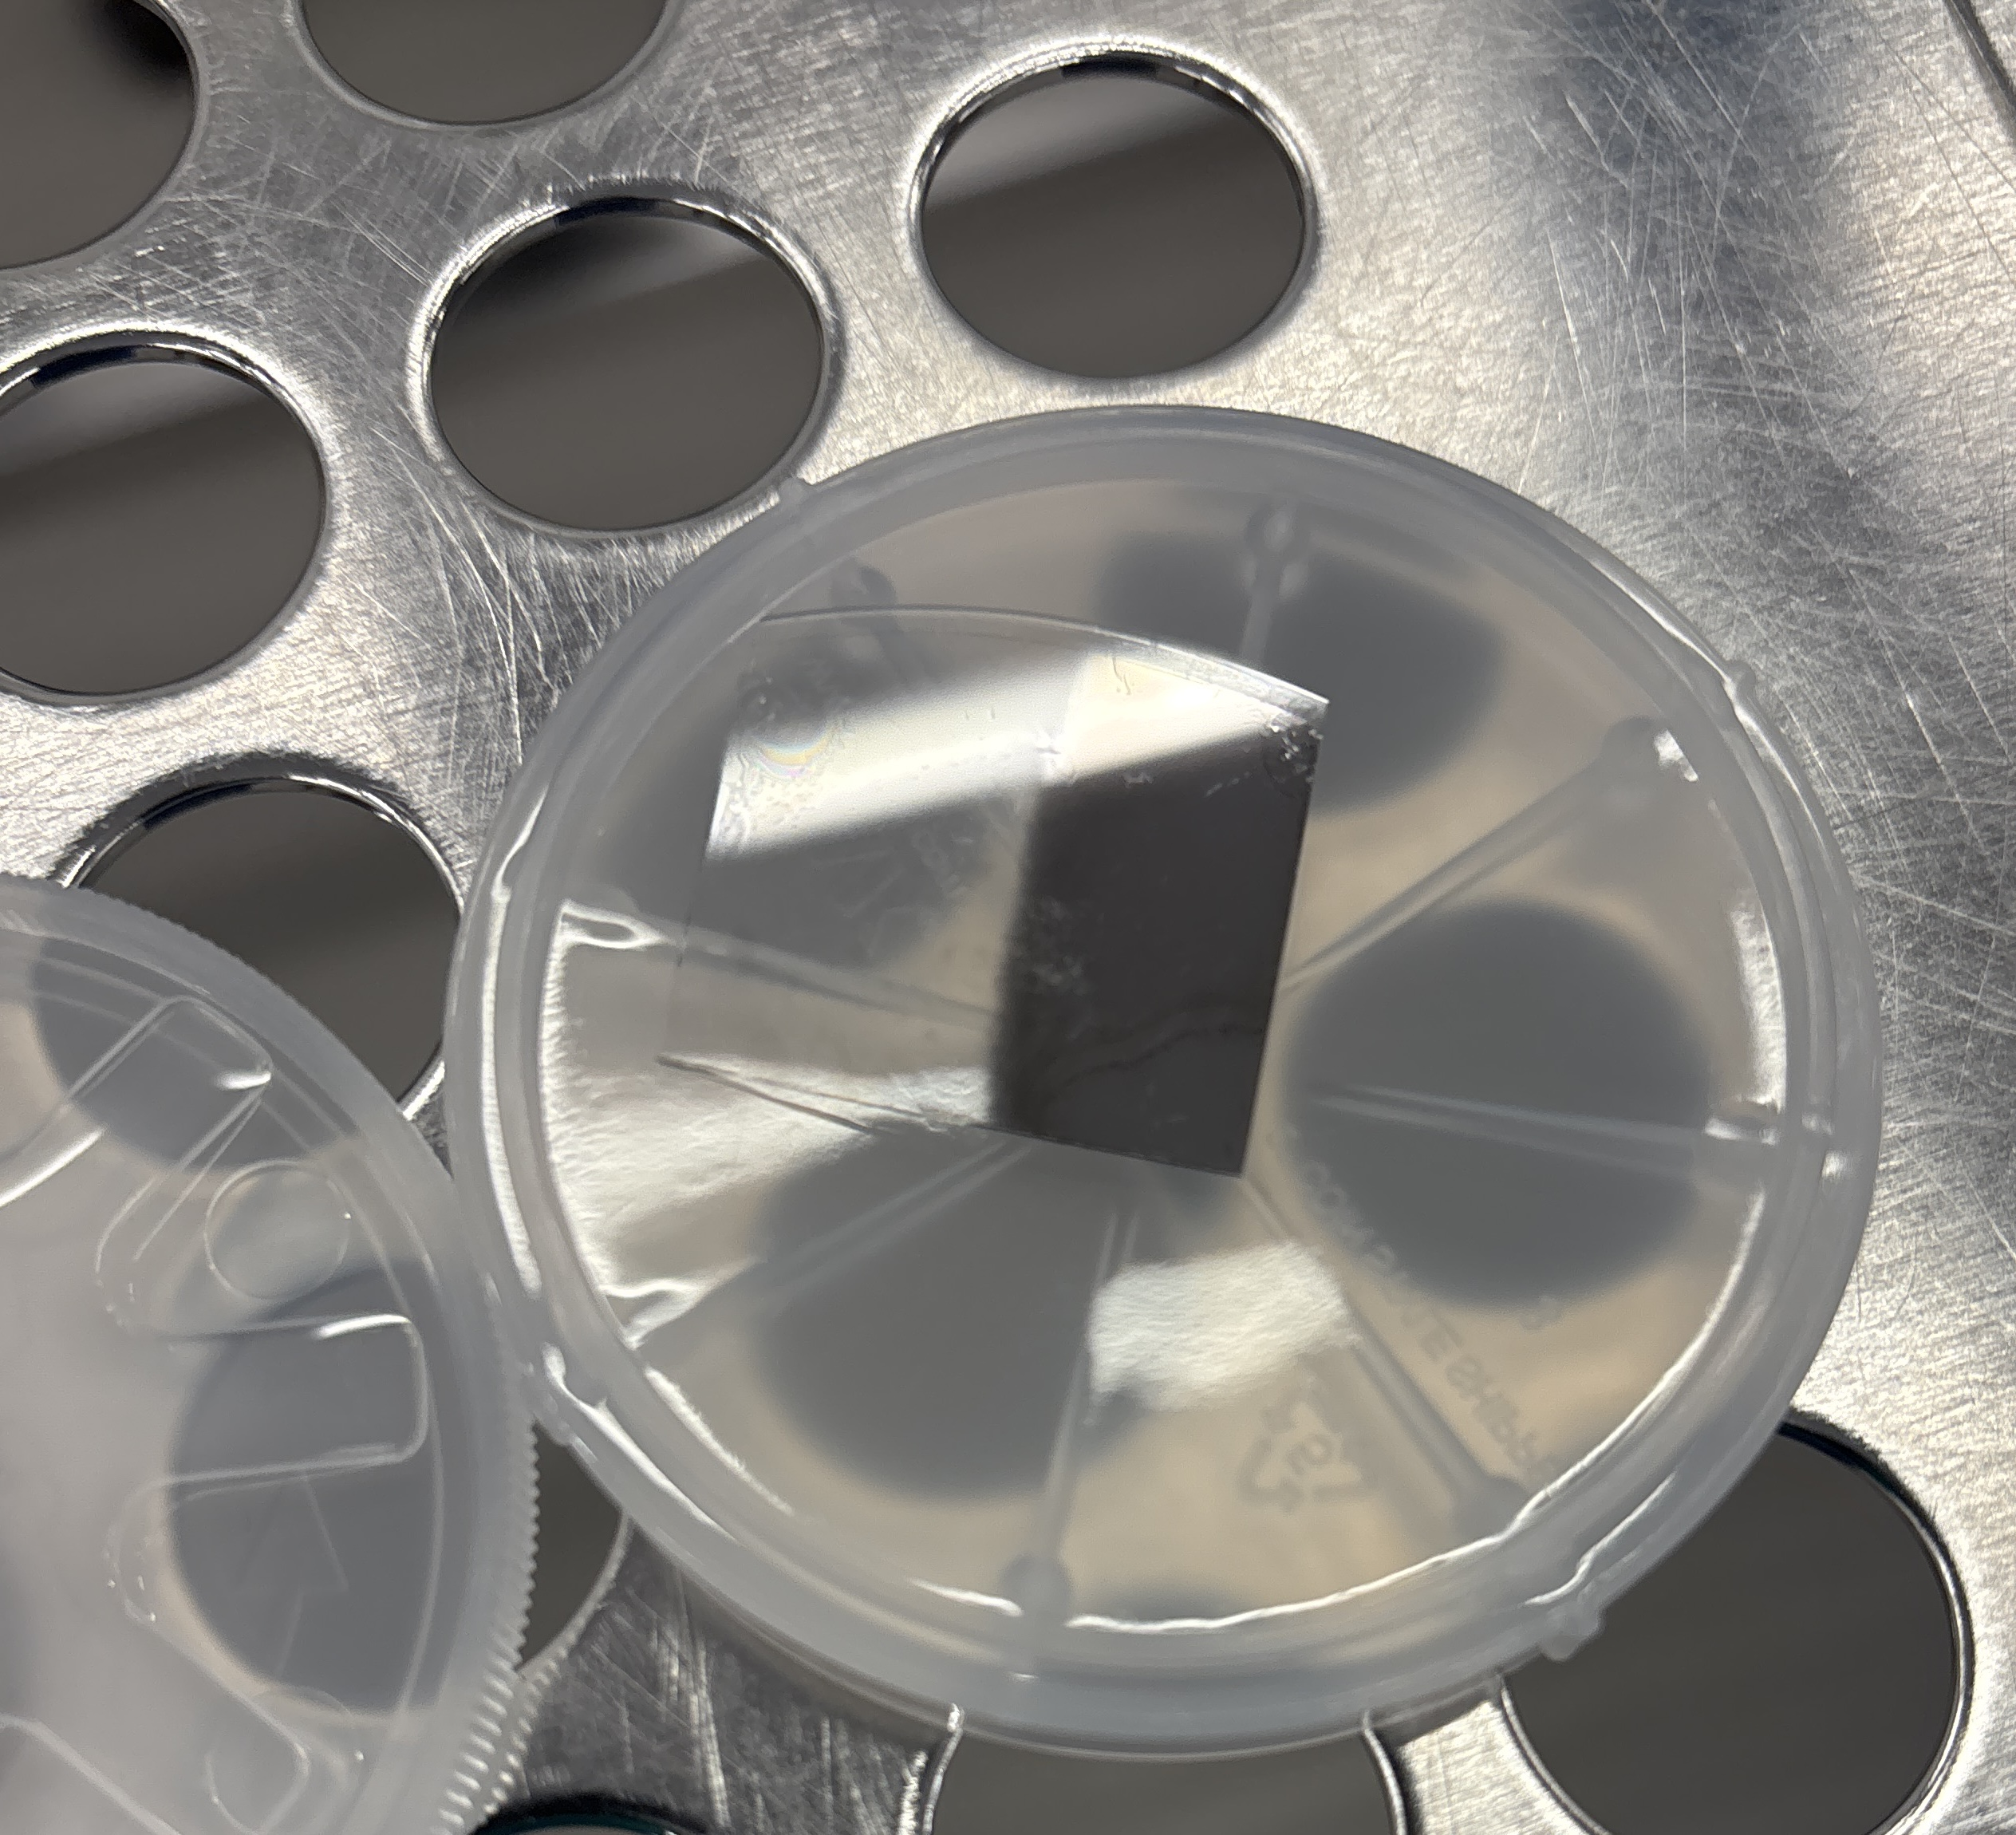
\includegraphics[width=0.6\textwidth]{figures/re_etched_away/re_etched_piranha.jpg}
    \caption{Visual evidence of an 80\% Re / 20\% Ta thin film completely etched away by a standard piranha solution clean, revealing the underlying sapphire substrate. This indicates that a 20\% Ta concentration is insufficient to passivate the alloy against aggressive acid treatments typically survived by pure Ta.}
    \label{fig:piranha_etch}
\end{figure}

XPS data on Ta and Re was then taken in weekly intervals. Control samples (approximately 6 months of ambient exposure) were kept and measured for comparison. Following XPS collection, scanning electron microscopy data was collected to confirm the structural changes. As shown in Figure \ref{Tantalum oxide growth vs. control}, even uncorrected spectra showed clear growth.

\begin{figure}[H]
     \centering
     \begin{subfigure}{0.45\textwidth}
         \centering
         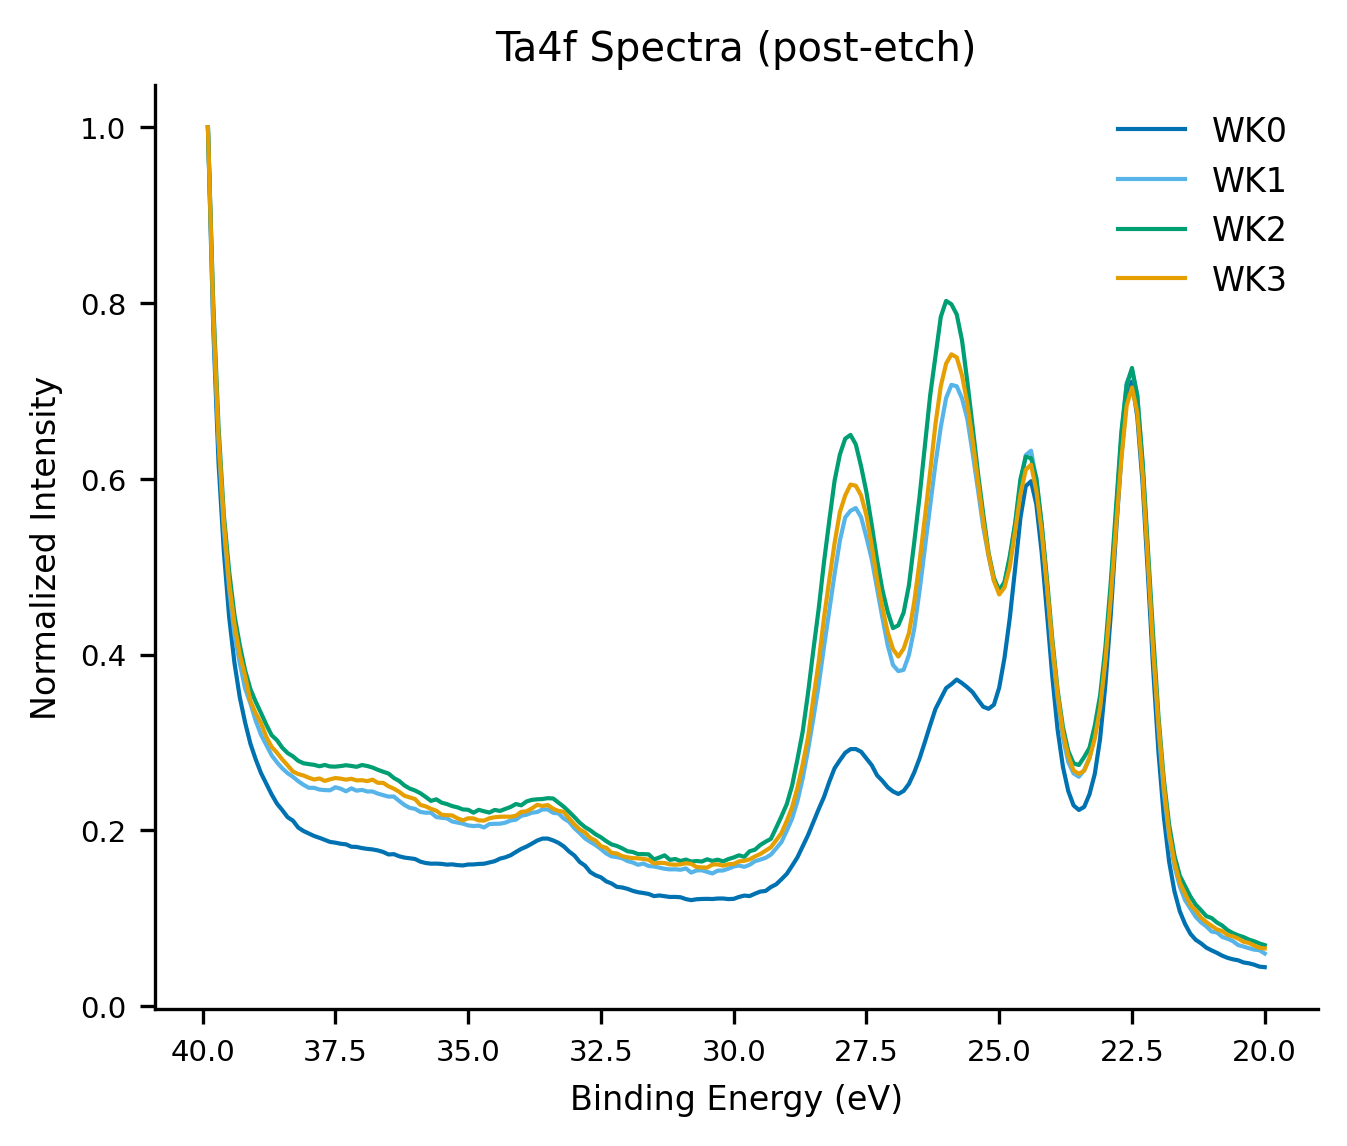
\includegraphics[width=\textwidth]{figures/raw_spectra/ta4f_postetch_overlay.png}
     \end{subfigure}
     \begin{subfigure}{0.45\textwidth}
         \centering
         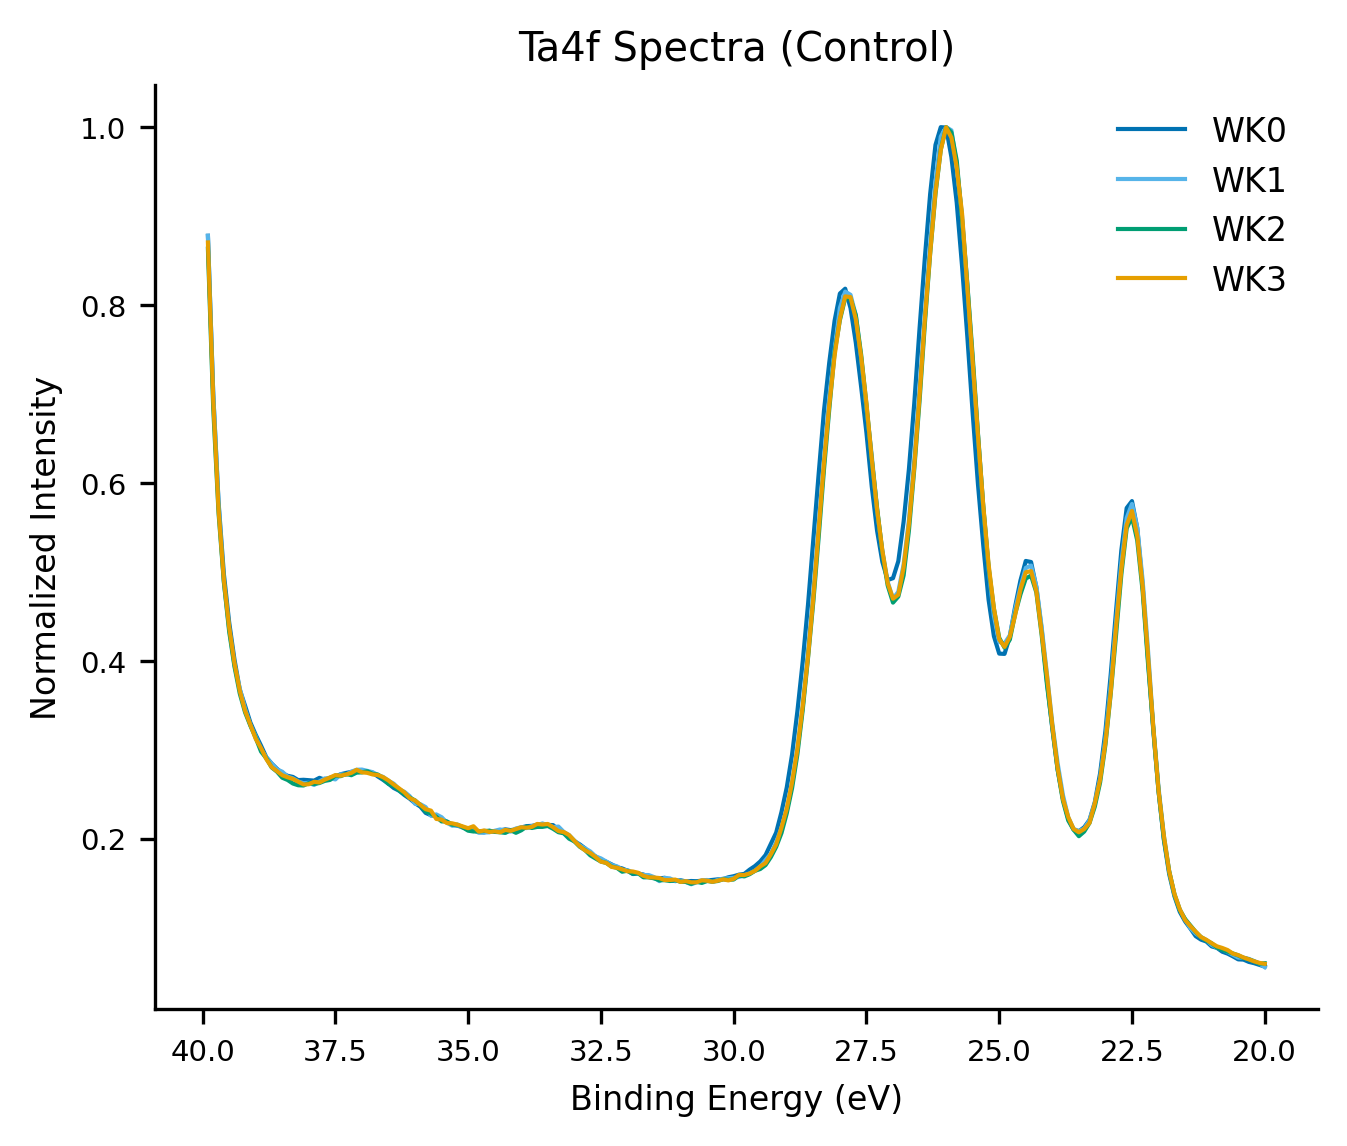
\includegraphics[width=\textwidth]{figures/raw_spectra/ta4f_control_overlay.png}
     \end{subfigure}
     \begin{subfigure}{0.45\textwidth}
         \centering
         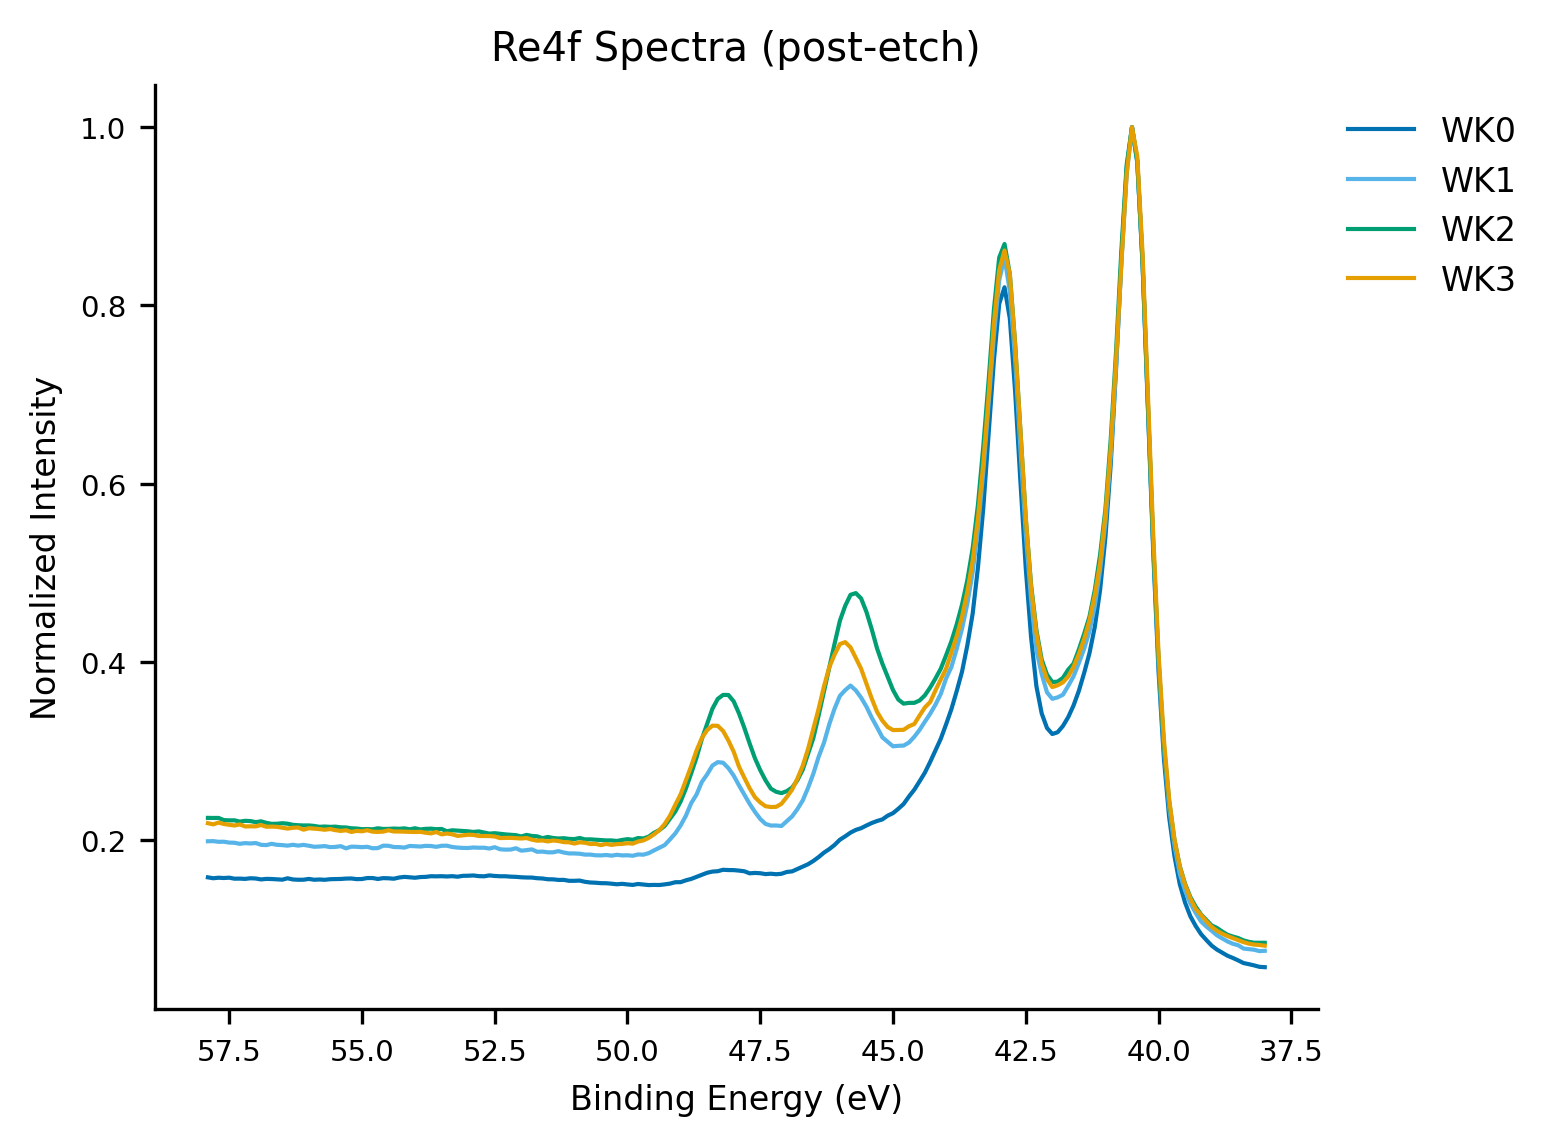
\includegraphics[width=\textwidth]{figures/raw_spectra/re4f_postetch_overlay.png}
     \end{subfigure}
     \begin{subfigure}{0.45\textwidth}
         \centering
         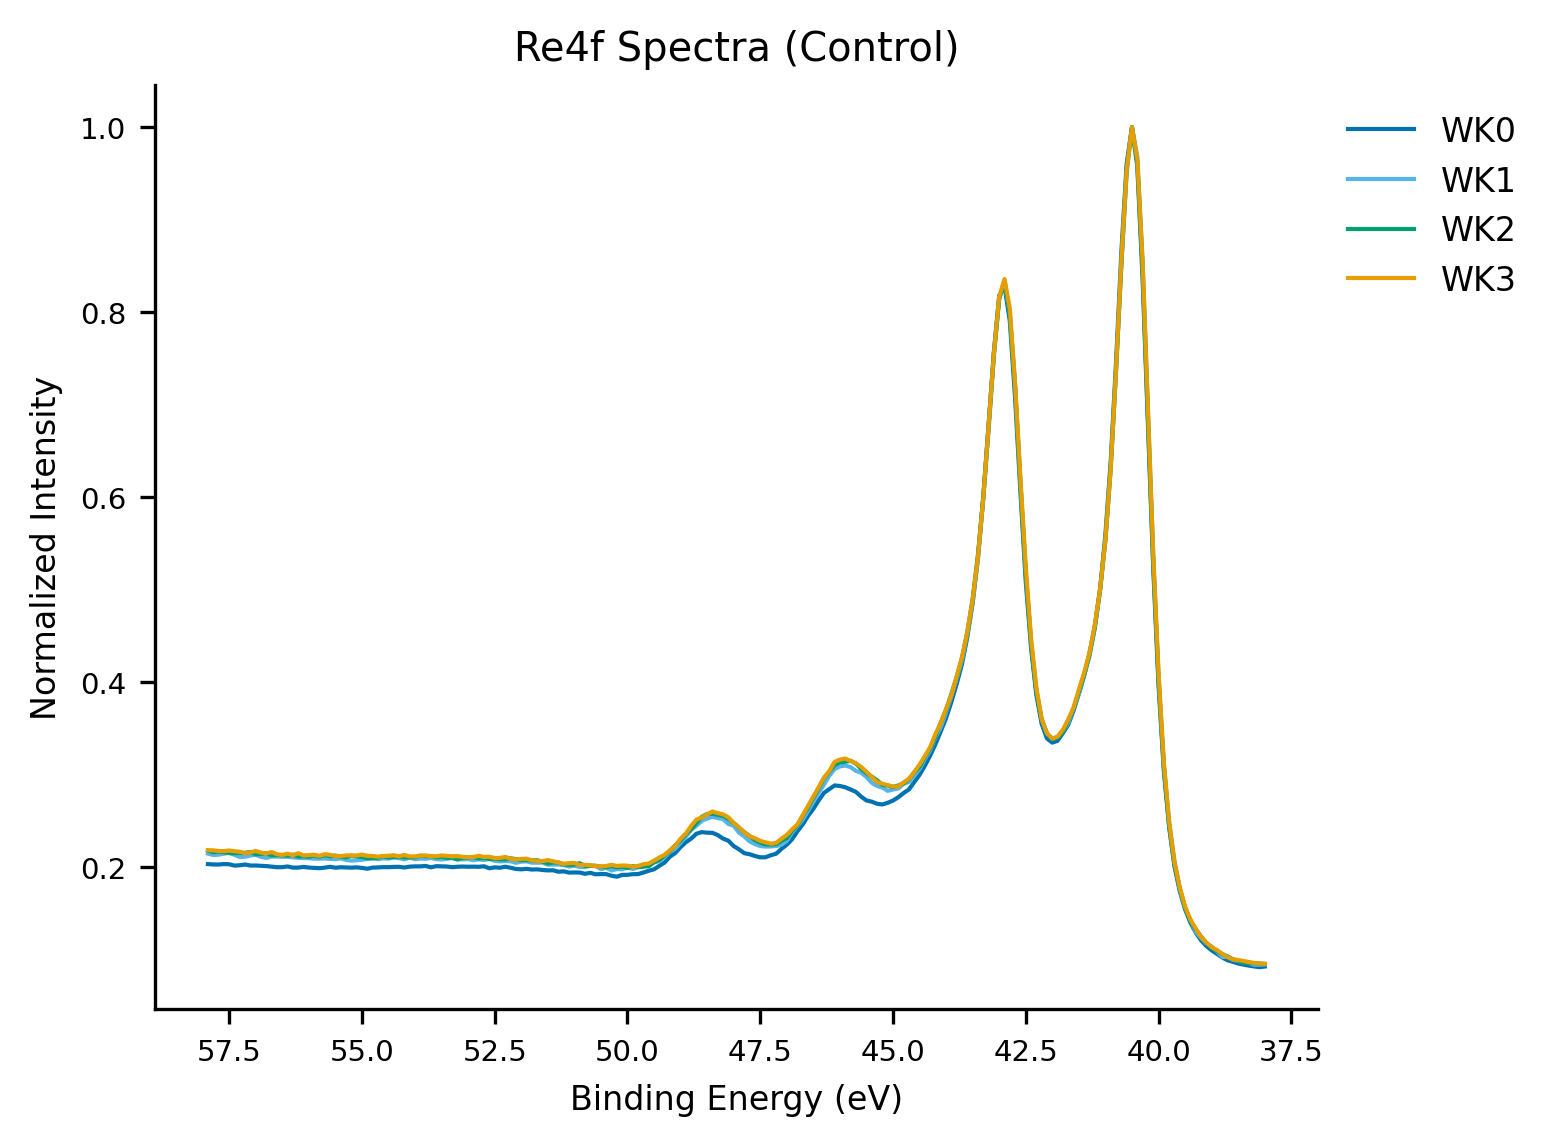
\includegraphics[width=\textwidth]{figures/raw_spectra/re4f_control_overlay.png}
     \end{subfigure}
        \caption{Oxide growth vs.\ control}
        \label{Tantalum oxide growth vs. control}
\end{figure}

\subsection{Fitting Procedure}
Following Shirley background correction (0.01 cutoff and 0.2 eV step window), XPS intensities were area-normalized and peaks were fitted using an \texttt{lmfit} non-linear least-squares minimization procedure \cite{mclellan2023}\cite{greiner2014}. Each species was modeled as a doublet attributed to the $4f_{7/2}$ and $4f_{5/2}$ spin-orbit split energy levels.

For Ta4f core electron ionization in the 20 eV to 30 eV range, the model incorporated six distinct pairs of peaks: a $Ta^{0}$ metal bulk state, an interface state, an alloy-shifted state, and three progressive oxidation states ($Ta^{1+}$, $Ta^{3+}$, and $Ta^{5+}$ primarily corresponding to $\mathrm{Ta_2O_5}$). 

Similarly, for Re4f in the 40 eV to 50 eV range, the model was significantly more complex, encompassing $Re^{0}$ metal, three sub-surface oxygen-coordinated states ($Re^{\delta+}$ shifted at +0.22, +0.45, and +0.73 eV above $Re^{0}$), and distinct oxide phases corresponding to $ReO$ ($Re^{2+}$), $ReO_2$ ($Re^{4+}$), $ReO_3$ ($Re^{6+}$), and $Re_2O_7$ ($Re^{7+}$). Detailed fitting constraints for these levels, including spin-orbit splitting and branching ratios, are provided in the Appendix. 

To accurately capture the physics of the material surface, asymmetric components (such as metal, alloy, and interface states) were fitted using a Skewed Voigt lineshape to account for conduction electron screening. Conversely, symmetric Gaussian lineshapes were employed for the purely oxide phases.

It should be noted that these fitting parameters were developed primarily for pure Ta and pure Re systems; their applicability to a 80\% Re 20\% Ta alloy may be limited, and this constraint motivates several of the observations discussed in Section~\ref{sec:peakcomp}. Figure \ref{Sample XPS fits} shows sample fits for Ta and Re immediately following treatment with BOE. While most Ta data had data vs.\ fitting residuals $<0.005$, Re saw worse fits with residuals $<0.02$.

\begin{figure}[H]
     \centering
     \begin{subfigure}{0.45\textwidth}
         \centering
         
\includegraphics[width=\textwidth]{figures/fits/Ta4f_-_BOE_WK0.png}
     \end{subfigure}
     \begin{subfigure}{0.45\textwidth}
         \centering
         
\includegraphics[width=\textwidth]{figures/fits/Ta4f_-_Control_WK0.png}
     \end{subfigure}
    \begin{subfigure}{0.45\textwidth}
         \centering
         
\includegraphics[width=\textwidth]{figures/fits/Re4f_-_BOE_WK0.png}
     \end{subfigure}
     \begin{subfigure}{0.45\textwidth}
         \centering
         
\includegraphics[width=\textwidth]{figures/fits/Re4f_-_Control_WK0.png}
     \end{subfigure}
        \caption{Sample XPS fits}
        \label{Sample XPS fits}
\end{figure}

After normalizing data based on the total intensity under the curve, proportions of each species relative to the whole surface were extracted in Figure \ref{area_fractions}. Similar to pure Ta films, we found $Ta_2O_5$ grows to become the dominant suboxide species of tantalum. With Re, however, $Re_2O_7$ seems to see significant growth over the first few weeks but takes up less of the oxide surface after saturation.

\begin{figure}[H]
     \centering
     \begin{subfigure}{\textwidth}
         \centering
         
\includegraphics[width=0.65\textwidth]{figures/area_fractions/ta4f_stacked_fractions.png}
         \subcaption{Tantalum species}
     \end{subfigure}
     \begin{subfigure}{\textwidth}
         \centering
         
\includegraphics[width=0.65\textwidth]{figures/area_fractions/re4f_stacked_fractions.png}
         \subcaption{Rhenium species}
     \end{subfigure}
        \caption{Tantalum vs.\ Rhenium oxide species}
        \label{area_fractions}
\end{figure}

\subsection{Fitting Quality and Constraint Diagnostics}
To quantitatively assess the goodness-of-fit across the complex multi-species models, reduced $\chi^2$ statistics were extracted for all scans (Table \ref{tab:fitting_stats}). Overall, the fits maintained stable $\chi^2$ values across the timecourse, though variations indicate the models' differing efficacies in capturing the exact physical lineshapes of BOE-treated versus heavily oxidized control samples.

\begin{table}[H]
    \centering
    \begin{tabular}{lcc}
        \toprule
        \textbf{Sample} & \textbf{Ta4f Reduced $\chi^2$} & \textbf{Re4f Reduced $\chi^2$} \\
        \midrule
        BOE\_WK0     & 5.71 & 7.24 \\
        BOE\_WK1     & 6.42 & 6.29 \\
        BOE\_WK2     & 6.27 & 7.29 \\
        BOE\_WK3     & 6.00 & 6.50 \\
        Control\_WK0 & 8.11 & 4.56 \\
        Control\_WK1 & 8.40 & 5.51 \\
        Control\_WK2 & 6.79 & 5.39 \\
        Control\_WK3 & 7.05 & 4.62 \\
        \bottomrule
    \end{tabular}
    \caption{Reduced $\chi^2$ goodness-of-fit statistics across all samples.}
    \label{tab:fitting_stats}
\end{table}

Additionally, to verify that the large binding energy shifts observed (particularly for the $\mathrm{Ta_2O_5}$ state) were not artefacts of optimizer constraint boundaries, an unconstrained free-fitting diagnostic was performed on the BOE\_WK0 sample. After relaxing the $\mathrm{Ta^{5+}}$ center constraint bounds from [25.5, 28.0] eV to [24.0, 29.0] eV, the fit naturally converged at $25.88 \pm 0.01$ eV. As seen in Figure \ref{fig:ta5_constraint_check}, this clean convergence nearly 1 eV below the expected pure-Ta position of 26.8 eV confirmed that the observed deviation represents a real initial-state chemical shift rather than a fitting artefact or misidentified sub-oxide state, motivating the deeper investigation of binding energy shifts in Section \ref{sec:peakcomp}.

\begin{figure}[H]
    \centering
    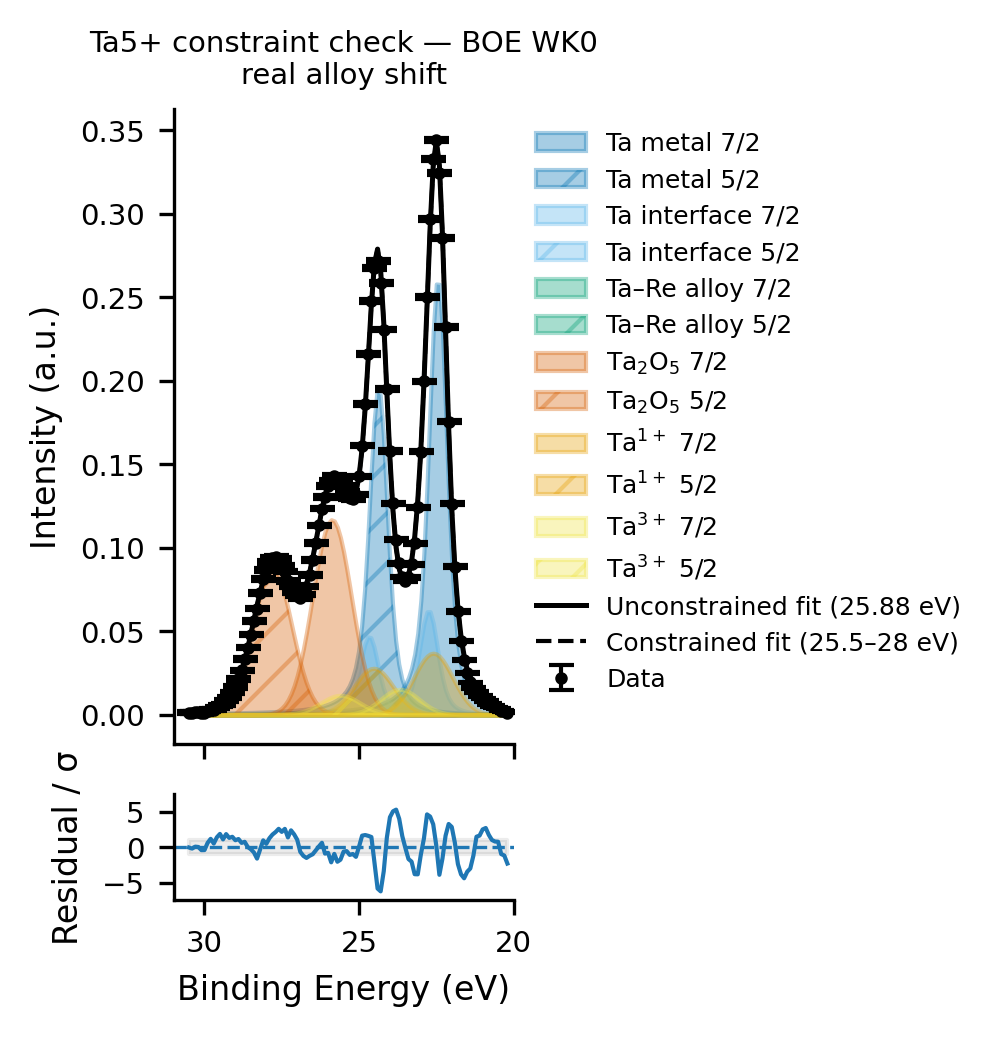
\includegraphics[width=0.65\textwidth]{figures/fits/ta5_constraint_check_boe_wk0.png}
    \caption{Diagnostic unconstrained fit of the Ta4f core level for the BOE\_WK0 sample. The $\mathrm{Ta^{5+}}$ peak naturally converges at $25.88$ eV, significantly shifted from the standard $\mathrm{Ta_2O_5}$ position ($26.8$ eV), confirming a genuine chemical shift.}
    \label{fig:ta5_constraint_check}
\end{figure}

\subsection{Thickness Estimation}
Following fitting, a very rough estimate of the surface layer was taken using the Strohmeier overlayer model. While more thorough estimation may require variable energy XPS or other methods, Strohmeier assumes the oxide surface is a uniform layer on top of the metal, attenuating the photoelectron signal from the underlying metal based on exponential decay. (It does not account for compositional gradients, surface roughness, etc.\cite{Strohmeier1990ESCA}.)

\begin{equation}
d = \lambda_{\mathrm{ox}} \cos\theta \;
\ln\!\left[
1 + \frac{I_{\mathrm{ox}}}{I_{\mathrm{m}}}
\left(\frac{S_{\mathrm{m}}}{S_{\mathrm{ox}}}\right)
\left(\frac{N_{\mathrm{m}}}{N_{\mathrm{ox}}}\right)
\right]
\label{eq:strohmeier}
\end{equation}

In the expression, \( d \) represents the oxide thickness, \( \lambda_{\mathrm{ox}} \) the effective inelastic mean free path (IMFP) of photoelectrons in the oxide, and \( \theta \) the photoelectron take-off angle relative to the surface. \( I_{\mathrm{ox}} \) and \( I_{\mathrm{m}} \) represent the (background-corrected) XPS peak areas associated with the oxide and metallic chemical states, respectively, while the factors \( S_{\mathrm{ox}} \) and \( S_{\mathrm{m}} \) are the photoionization sensitivity factors for the corresponding oxide and metal signals. Finally, \( N_{\mathrm{ox}} \) and \( N_{\mathrm{m}} \) denote the atomic number densities of the elements.

For this experiment, the X-ray source/collector was normal to the plane while the oxide and metal contributions originated from the same core level of the same element. Under these assumptions, Eq.~\ref{eq:strohmeier} reduced to the form

\begin{equation}
d \approx \lambda_{\mathrm{ox}} \cos\theta \;
\ln\!\left[
1 + \frac{I_{\mathrm{ox}}}{I_{\mathrm{m}}}
\left(\frac{N_{\mathrm{m}}}{N_{\mathrm{ox}}}\right)
\right].
\label{eq:strohmeier_simplified}
\end{equation}

Using Eq.~\ref{eq:strohmeier_simplified}, the apparent oxide thicknesses associated with both the tantalum and rhenium components were calculated independently. It must be noted here that the Strohmeier model to individual components of an alloy carries significant limitations; the model assumes a uniform, pure oxide overlayer on a pure metal substrate. In a Ta-Re alloy, the surface is a mixed or stratified oxide, meaning Re metal photoelectrons are attenuated by the entire mixed-oxide layer, not just Re oxides. These independent calculations yield ``equivalent effective thicknesses'' rather than absolute depths of the oxide-metal interface. Yet even with these limitations, Ta dominates the surface oxide network such that the Ta-derived thickness serves as a reasonable proxy for the total oxide layer thickness, while the Re-derived thickness quantifies the relative extent of Re oxidation within that layer.

For the control samples, the equivalent tantalum oxide thickness was consistently around 3.3--3.4~nm, while the equivalent rhenium oxide was very thin, measuring roughly 0.55~nm. Following BOE treatment, the initial equivalent oxide thicknesses (WK0) were substantially reduced to 1.39~nm for Ta and 0.34~nm for Re. 

Over the subsequent three weeks of ambient exposure, both oxide species exhibited significant regrowth. To quantify the oxidation kinetics, the time-course thickness data for the BOE-treated samples were fitted to a Cabrera-Mott growth model:
\begin{equation}
x(t) = x_0 + k \ln\left(1 + \frac{t}{\tau}\right)
\label{eq:cabrera_mott}
\end{equation}
$x_0$ is the initial thickness, $k$ is the rate constant, and $\tau$ is a characteristic time constant. 

As shown in Figure~\ref{fig:cabrera_mott_fits}, the logarithmic model shows rapid initial re-oxidation followed by a slower saturation regime. For tantalum, the oxide regrew to roughly 2.4~nm by week 2, remaining noticeably thinner than the native control oxide ($\sim$3.4~nm). The Cabrera-Mott fit for Ta yielded $x_0 = 1.39 \pm 1.00$~nm, $k = 0.19 \pm 1.34$~nm, and $\tau = 0.01 \pm 0.47$~weeks. While the uncertainty bounds are broad due to the limited timepoints, the functional form describes the observed stabilization.

Interestingly, the equivalent rhenium oxide on the BOE-treated samples grew from 0.34~nm to approximately 1.21~nm by week 2 (with fit parameters $x_0 = 0.34 \pm 1.00$~nm, $k = 0.10 \pm 1.28$~nm, and $\tau = 0.001 \pm 0.10$~weeks). These differing growth profiles indicate a highly coupled, two-stage oxidation process within the alloy matrix. In the first stage (rapid oxidation), the removal of the passivating layer exposes both metals to the ambient environment. Lacking immediate passivation, Rhenium oxidizes aggressively. By week 2, the equivalent Re oxide regrows to approximately 1.21~nm—drastically overshooting its stable native thickness on the control sample ($\sim$0.55~nm). 

However, in the second stage (matrix saturation and re-equilibration), the growing Tantalum oxide network saturates at roughly 2.4~nm and begins to effectively passivate the bulk surface \cite{mclellan2023}. Concurrently, the Rhenium oxide thickness begins to shrink, dropping to 1.05~nm in week 3 and eventually reaching the much thinner state observed in the 6-month control. This kinetic overshoot suggests that once the dominant $\mathrm{Ta_2O_5}$ matrix forms and stabilizes, it halts further Re oxidation. The excess Re oxide that rapidly formed during the unpassivated first stage is subsequently expelled, volatilized, or dissolved from the stabilizing Ta matrix, highlighting that the Ta-Re surface is not a static layer but a system striving toward a complex chemical equilibrium over several months.

\begin{figure}[H]
    \centering
    \begin{subfigure}{\textwidth}
        \centering
        
\includegraphics[width=0.65\textwidth]{figures/thickness/ta_cabrera_mott_fit.png}
        \caption{Tantalum Oxide}
    \end{subfigure}\hfill
    \begin{subfigure}{\textwidth}
        \centering
        
\includegraphics[width=0.65\textwidth]{figures/thickness/re_cabrera_mott_fit.png}
        \caption{Rhenium Oxide}
    \end{subfigure}
    \caption{Cabrera-Mott logarithmic growth fits for Ta and Re equivalent oxide thicknesses on BOE-treated samples over a 3-week period.}
    \label{fig:cabrera_mott_fits}
\end{figure}

These findings confirm that BOE treatment is effective at nearly eliminating the oxide layer. The speed of growth is also notable; in general, the estimated Ta thicknesses are comparable to accepted values for native tantalum oxides even in an oxide with 80\% rhenium content ($\approx 2.257\pm 0.023$ nm) \cite{mclellan2023}. The persistent, evolving mixed-oxide layer is likely a significant source of loss when fabricated into devices.

\subsection{Binding Energy and Amplitude Shifts}
\label{sec:peakcomp}
Beyond thickness variations, the chemical speciation of the surface layer exhibited deviations from pure elemental references. Across both the time-course measurements and long-term control samples, fitted peak centers for various oxidation states shifted consistently, as shown in Figure \ref{fig:binding_energy_evolution}. Metallic Ta 4f components exhibited a large positive binding energy (BE) shift ($\approx +0.42$ eV) relative to pure Ta metal, while metallic Re 4f shifted slightly positive ($\approx +0.10$ eV). Conversely, the primary tantalum oxide ($\mathrm{Ta}^{5+}$ in $\mathrm{Ta_2O_5}$) underwent a negative shift ($\approx -0.91$ eV) compared to its accepted standard position. With Re, the rhenium oxides ($\mathrm{Re}^{4+}$, $\mathrm{Re}^{6+}$, $\mathrm{Re}^{7+}$) exhibited positive shifts ranging from $+0.3$ to $+0.6$ eV. 

\begin{figure}[H]
     \centering
     \begin{subfigure}{\textwidth}
         \centering
         
\includegraphics[width=0.65\textwidth]{figures/shifts/ta4f_binding_energy_evolution_by_species.png}
         \caption{Tantalum BE Evolution}
     \end{subfigure}\hfill
     \begin{subfigure}{\textwidth}
         \centering
         
\includegraphics[width=0.65\textwidth]{figures/shifts/re4f_binding_energy_evolution_by_species.png}
         \caption{Rhenium BE Evolution}
     \end{subfigure}
        \caption{Time evolution of binding energy deviations ($\Delta$ eV) from expected pure-element references for Ta and Re species across BOE-treated and control samples.}
        \label{fig:binding_energy_evolution}
\end{figure}

The opposing nature of these shifts---where oxidized Ta shifts negatively while oxidized Re shifts positively---is summarized in Figure \ref{fig:be_correlation}. This systematic, opposing movement across the entire sample set strongly points toward a shared electronic environment rather than randomly misidentified independent oxide phases.

\begin{figure}[H]
    \centering
    
\includegraphics[width=0.65\textwidth]{figures/shifts/be_shift_ta_re_correlation.png}
    \caption{Correlation between Tantalum and Rhenium binding energy shifts relative to standard pure-element references. The opposing shifts (Ta negative, Re positive) are consistently maintained across the growth period and long-term control.}
    \label{fig:be_correlation}
\end{figure}

The amplitudes (relative concentrations) of these species also evolved dynamically. Most notably, as shown in Figure \ref{fig:amplitude_evolution}, the highly oxidized $\mathrm{Re_2O_7}$ state was nearly non-existent immediately post-etch ($<1\%$ of the Re signal). Over the next two weeks, it rapidly grew to comprise $\approx 15\%$ of the Re signal. However, in the 6-month control sample, this fraction was significantly reduced to roughly 4--5\%. This chemical speciation directly explains the thickness "overshoot" observed in the Re oxide timecourse. The initial burst of unpassivated oxidation heavily favors the formation of high-state $\mathrm{Re^{7+}}$ ($\mathrm{Re_2O_7}$). However, $\mathrm{Re_2O_7}$ is known to be highly volatile and hygroscopic, converting readily to perrhenic acid upon exposure to ambient moisture \cite{cimino1980photoelectron, greiner2014}. Thus, as the surrounding $\mathrm{Ta_2O_5}$ matrix saturates and passivates the surface, this unstable, highly oxidized $\mathrm{Re^{7+}}$ phase is selectively lost to the environment. The eventual thinning and stabilization of the Re oxide layer is physically driven by the departure of this specific $\mathrm{Re_2O_7}$ component, leaving behind a thinner, lower-oxidation-state Re matrix embedded within the passivating Tantalum oxide.

\begin{figure}[H]
     \centering
     \begin{subfigure}{\textwidth}
         \centering
         
\includegraphics[width=0.65\textwidth]{figures/shifts/ta4f_amplitude_evolution_by_species.png}
         \caption{Tantalum Amplitude Evolution}
     \end{subfigure}\hfill
     \begin{subfigure}{\textwidth}
         \centering
         
\includegraphics[width=0.65\textwidth]{figures/shifts/re4f_amplitude_evolution_by_species.png}
         \caption{Rhenium Amplitude Evolution}
     \end{subfigure}
        \caption{Evolution of normalized XPS peak amplitudes for individual Ta and Re oxidation states across BOE-treated and control samples.}
        \label{fig:amplitude_evolution}
\end{figure}

\subsection{Further Morphology}
\label{sec:morphology}
Scanning Electron Microscopy (SEM) imaging was performed on a control sample (6 months of ambient exposure) to confirm the sample structure.

\begin{figure}[H]
    \centering
    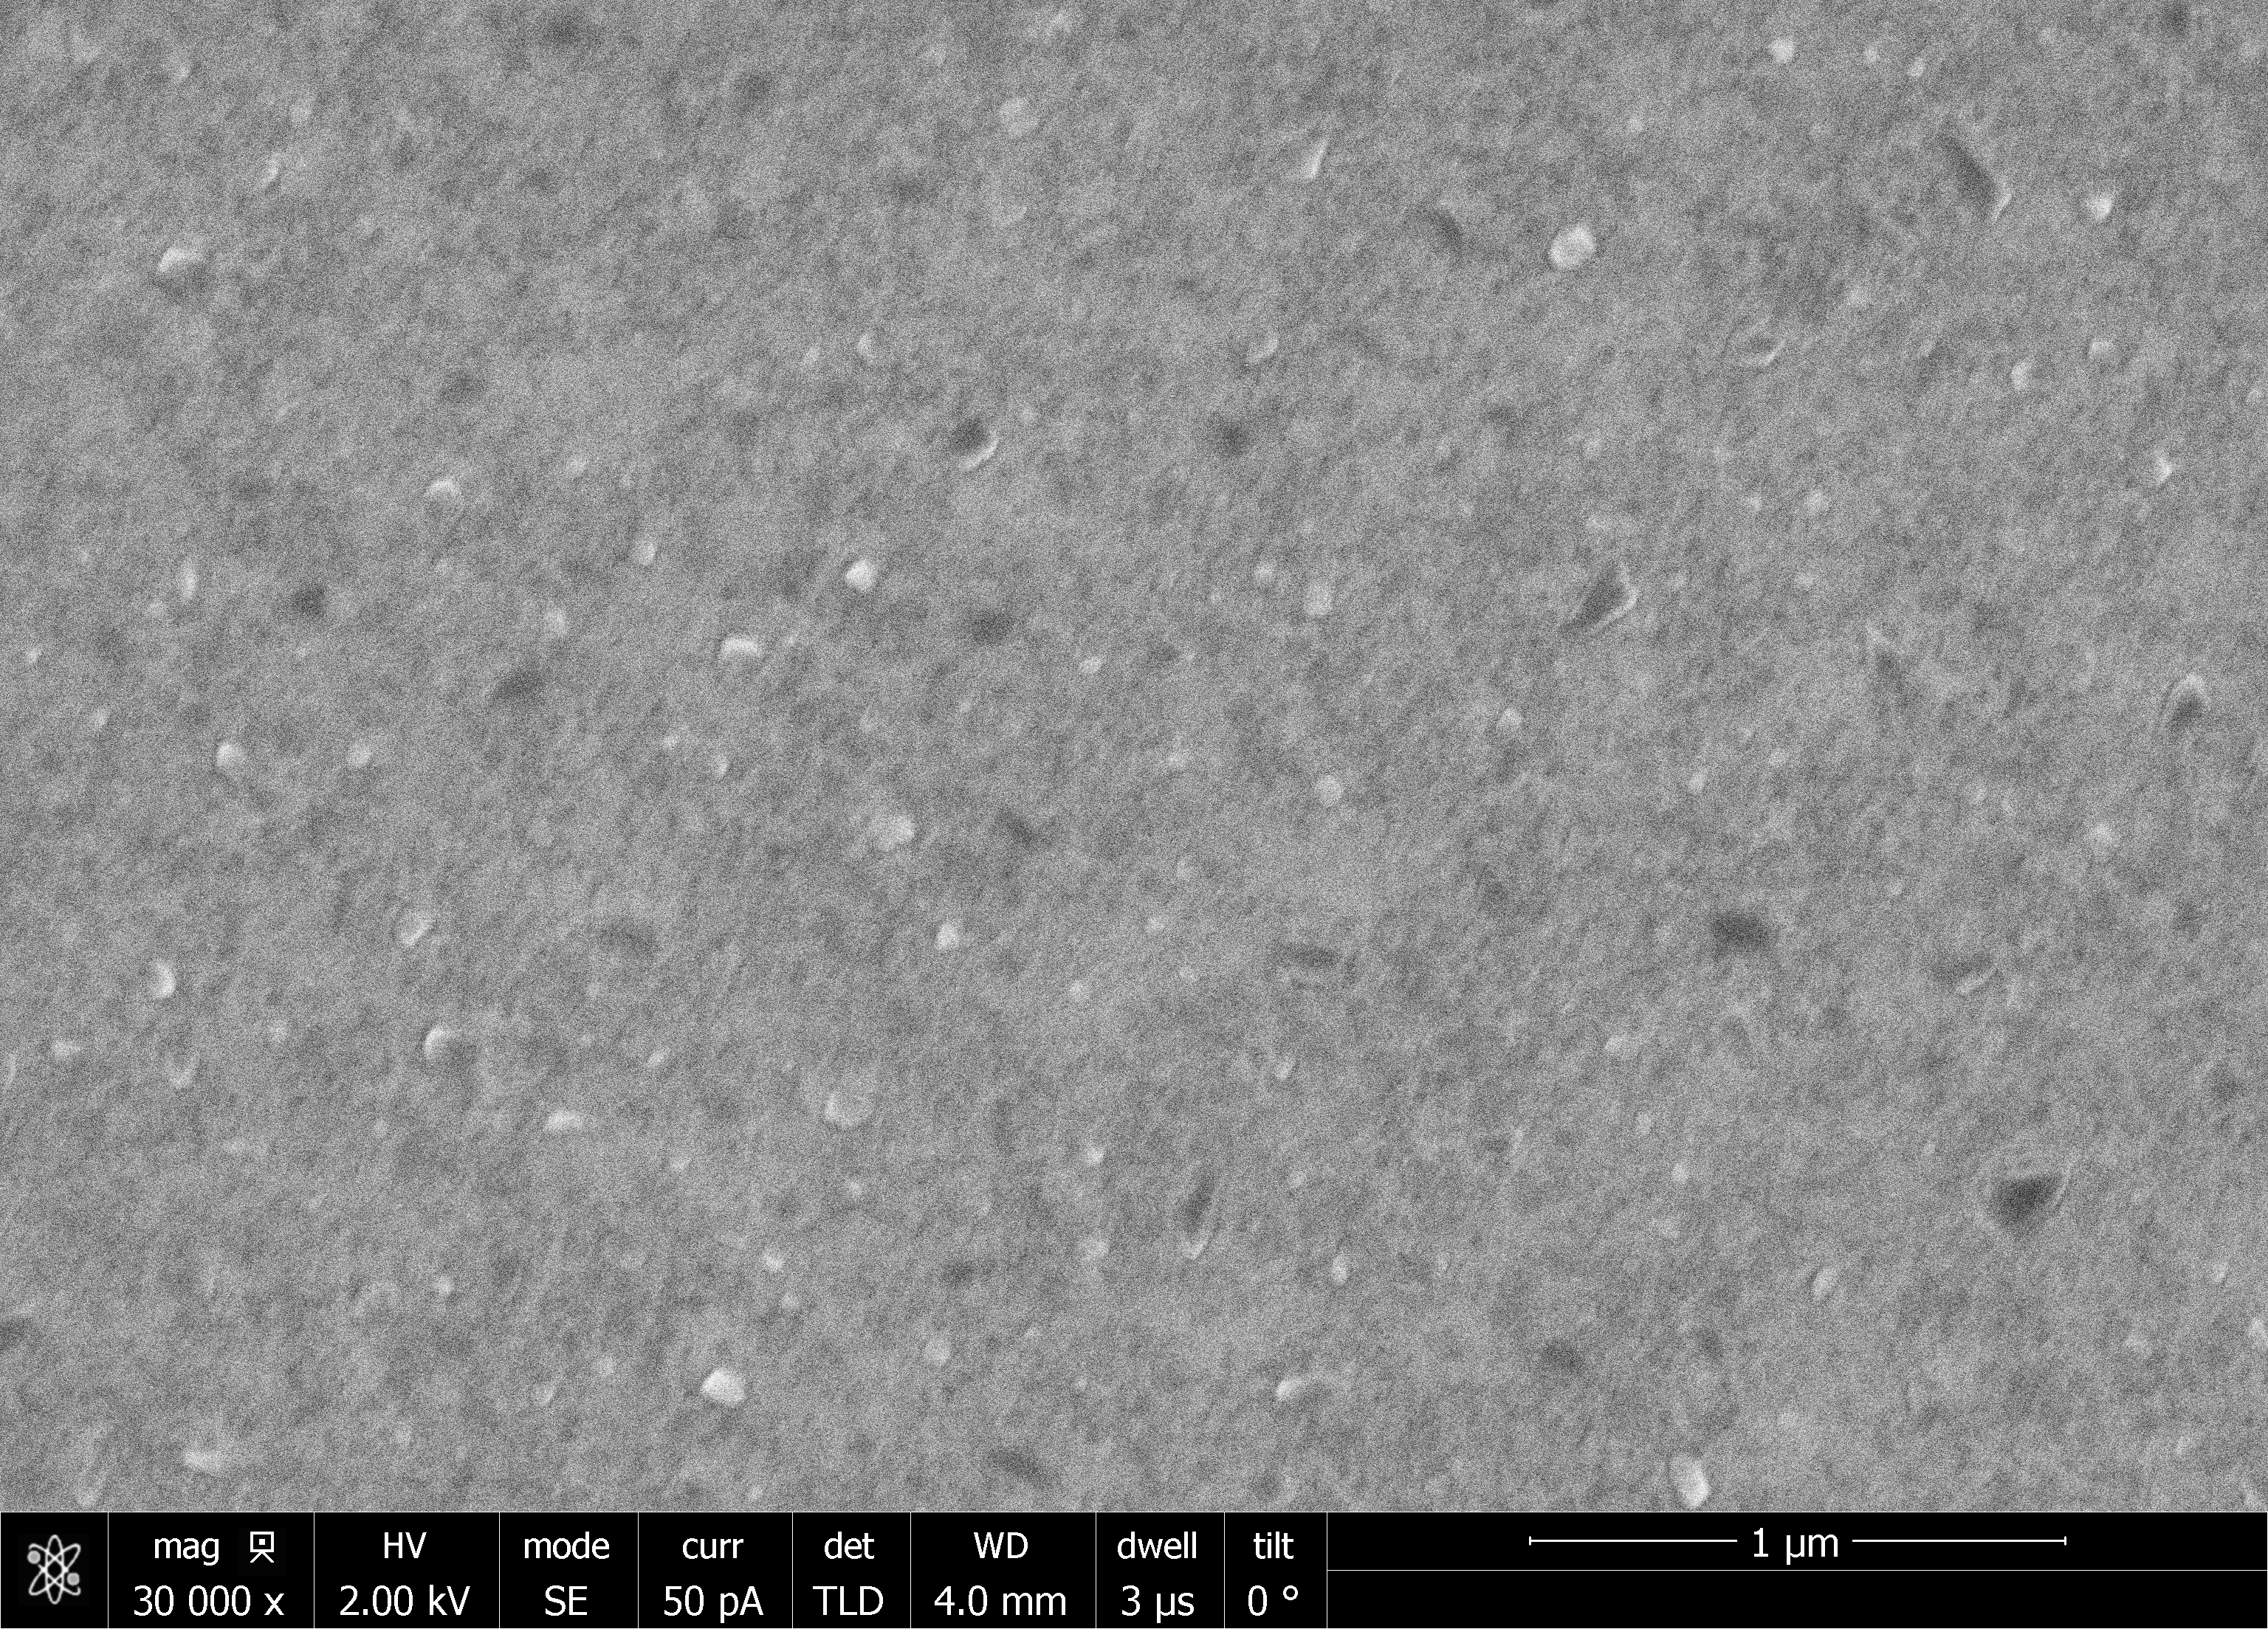
\includegraphics[width=0.65\textwidth]{figures/sem_surface_morphology.png}
    \caption{SEM image of the TaRe thin film surface, revealing the surface topography and morphology of the native oxide layer.}
    \label{fig:sem_morphology}
\end{figure}

Although contamination of sample is apparent in the image, (likely arising from handling and ambient exposure during the exposure period), the underlying surface appears amorphous with botches of uneven morphology.

To further probe the crystalline phases of the oxide layer, an initial grazing incidence X-ray diffraction (GIXRD) analysis was performed on the film. However, the diffractogram was overwhelmingly dominated by the massive reflections of sapphire ($\alpha$-Al$_2$O$_3$) substrate located at $2\theta \approx 41.6^\circ$ and $90.6^\circ$, respectively. Consequently, very few discernible diffraction peaks could be attributed to the TaRe thin film or its native oxides. 

While more careful analysis might yield a cleaner signal, the absence of crystalline oxide peaks corroborates the XPS data, indicating that the native oxide layer (Ta$_2$O$_5$ and suboxides) is substantially amorphous. This lack of long-range crystalline order within the oxide implies a highly disordered dielectric medium that commonly hosts TLS defects.

\begin{figure}[H]
    \centering
    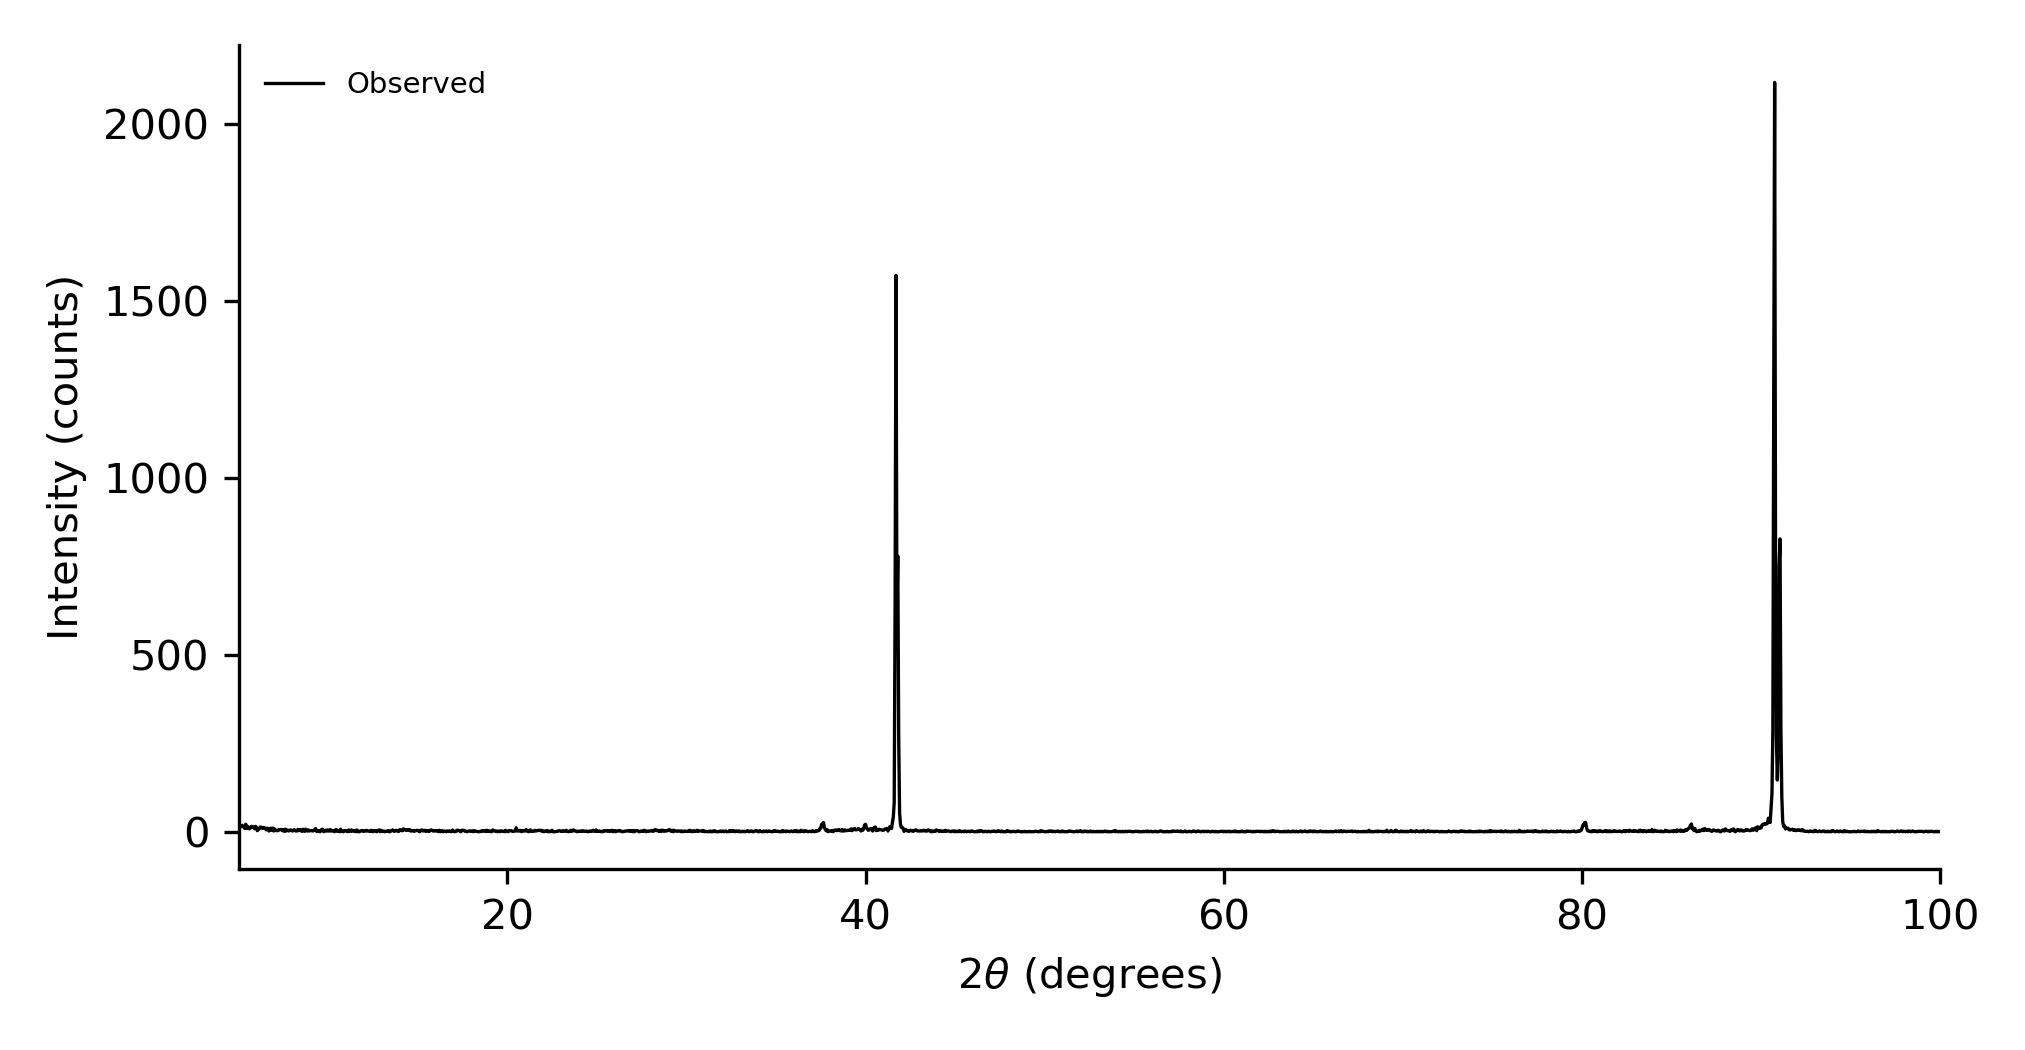
\includegraphics[width=0.65\textwidth]{figures/TaRe_Full_Oxide_quicklook.png}
    \caption{Raw grazing incidence X-ray diffraction (GIXRD) diffractogram of the TaRe thin film, demonstrating the dominance of the sapphire substrate peaks and the lack of distinct crystalline oxide phases.}
    \label{fig:gixrd_raw}
\end{figure}

\section{Discussion and Next Steps}
This analysis reveals several key features regarding the general growth dynamics of the native oxide on Ta-Re alloys. Most notably, the timecourse data illustrates a coupled, two-stage oxidation process following the initial removal (or "reset") of the surface via Buffered Oxide Etch (BOE). In the first stage, unpassivated rhenium oxidizes aggressively, rapidly forming a thick oxide layer dominated by the $\mathrm{Re^{7+}}$ state ($\mathrm{Re_2O_7}$). This leads to a thickness "overshoot" compared to the native equilibrium state shown in the control. In the second stage, the formation of the self-limiting $\mathrm{Ta_2O_5}$ network saturates and passivates the surface \cite{mclellan2023}. Because $\mathrm{Re_2O_7}$ is highly volatile and hygroscopic \cite{cimino1980photoelectron, greiner2014}, it is subsequently dissolved or expelled from the stabilizing matrix. The result is an eventual re-equilibration where the effective rhenium oxide thickness shrinks back down, embedded within a stable Ta-dominant matrix.

This dynamic two-stage growth behavior has significant implications for qubit fabrication. The transient, highly-oxidized state of $\mathrm{Re_2O_7}$ observed during the early growth phase poses a risk as a potential source of TLS dielectric loss; amorphous oxides and fluctuating charge traps associated with such unstable intermediate phases can easily absorb microwave energy, leading to decoherence \cite{crowley2023, mclellan2023}. Fabrication workflows for Ta-Re based circuits must either allow sufficient time,employ annealing to let the surface reach thermodynamic equilibrium, or use immediate in-vacuum passivation techniques to prevent the aggressive initial Re oxidation entirely.

The opposing binding energy shifts within the alloy also provide a strong indication of the underlying chemical structure. Because Re is significantly more electronegative than Ta (Pauling scale: 1.9 vs. 1.5), charge transfer naturally occurs from Ta to Re within the 80:20 alloy matrix. This depletion of local electron density around Ta causes its core-level electrons to become more tightly bound, potentially explaining the large $+0.42$ eV initial-state shift observed for the Ta metal peak. Importantly, the systemic and stable nature of these shifts across both the 3-week growth period and the 6-month control rules out the possibility that these deviations are simply misidentified pure oxide species. If the surface consisted of independent, non-interacting $\mathrm{Ta_2O_5}$ and Rhenium oxide domains, their binding energies would align closely with standard elemental references. Instead, the persistent, opposing shifts may indicate the presence of a distinct ternary Ta-Re-O phase where charge is re-distributed across the mixed lattice.

More detailed analysis using non-destructive techniques like variable-energy XPS and cross-sectional transmission electron microscopy (TEM) is strongly warranted to verify these measurements and accurately construct a depth profile of the alloy surface, especially as standard Ar$^+$ ion sputtering was found to induce preferential oxygen reduction rather than cleanly removing the oxide (see Appendix B). All code and data from this analysis are available in the accomanying GitHub repository \url{https://github.com/dandan002/TaRe-Analysis-Code.git}.


\newpage
\addcontentsline{toc}{section}{References}
\printbibliography

\newpage
\addcontentsline{toc}{section}{Appendix A: Fitting Constraints and Tables}
\section*{Appendix A: Fitting Constraints and Tables}
Detailed fitting constraints for the Ta4f and Re4f core levels were employed during non-linear least-squares minimization. For Ta4f core electron ionization in the 20 eV to 30 eV range, the spin-orbit splitting offset was constrained near 1.91 eV with a branching ratio of $\sim1.33$. For Re4f in the 40 eV to 50 eV range, the spin-orbit splitting was constrained between 2.35 and 2.50 eV with a $\sim1.33$ branching ratio. Asymmetric components were fitted using a Skewed Voigt lineshape to account for conduction electron screening, while symmetric Gaussian lineshapes were employed for purely oxide phases.

% -------------------- WK0 --------------------
\begin{table}[H]
\centering
\begin{threeparttable}
\caption{Fitted binding energies (WK0 - BOE)}
\begin{tabular}{llrrrr}
\toprule
Species & Spin & Expected (eV) & Fitted (eV) & StdErr (eV) & $\Delta$ (eV) \\
\midrule
\multicolumn{6}{l}{\textbf{BOE\_WK0}} \\
Ta metal & $7/2$ & 22.000 & 22.433 & 0.003 & 0.433 \\
Ta metal & $5/2$ & 23.900 & 24.343 & 0.003 & 0.443 \\
Ta interface & $7/2$ & 22.400 & 22.732 & 0.017 & 0.332 \\
Ta interface & $5/2$ & 24.300 & 24.642 & 0.017 & 0.342 \\
Ta alloy & $7/2$ & 24.000 & 24.933 & 0.003 & 0.933 \\
Ta alloy & $5/2$ & 25.900 & 26.843 & 0.003 & 0.943 \\
$\mathrm{Ta^{+1}}$ & $7/2$ & 22.700 & 22.600 & 0.056 & -0.100 \\
$\mathrm{Ta^{+1}}$ & $5/2$ & 24.600 & 24.510 & 0.056 & -0.090 \\
$\mathrm{Ta^{+3}}$ & $7/2$ & 24.200 & 23.675 & 0.107 & -0.525 \\
$\mathrm{Ta^{+3}}$ & $5/2$ & 26.100 & 25.585 & 0.107 & -0.515 \\
$\mathrm{Ta^{+5}}$ ($\mathrm{Ta_2O_5}$) & $7/2$ & 26.800 & 25.876 & 0.010 & -0.924 \\
$\mathrm{Ta^{+5}}$ ($\mathrm{Ta_2O_5}$) & $5/2$ & 28.700 & 27.786 & 0.010 & -0.914 \\
Re metal & $7/2$ & 40.350 & 40.456 & 0 & 0.106 \\
Re metal & $5/2$ & 42.770 & 42.888 & 0 & 0.118 \\
$\mathrm{Re}$ $\delta^{+1}$ & $7/2$ & 40.570 & 40.676 & 0 & 0.106 \\
$\mathrm{Re}$ $\delta^{+1}$ & $5/2$ & 42.990 & 43.108 & 0 & 0.118 \\
$\mathrm{Re}$ $\delta^{+2}$ & $7/2$ & 40.800 & 40.906 & 0 & 0.106 \\
$\mathrm{Re}$ $\delta^{+2}$ & $5/2$ & 43.220 & 43.338 & 0 & 0.118 \\
$\mathrm{Re}$ $\delta^{+3}$ & $7/2$ & 41.080 & 41.186 & 0 & 0.106 \\
$\mathrm{Re}$ $\delta^{+3}$ & $5/2$ & 43.500 & 43.618 & 0 & 0.118 \\
$\mathrm{ReO}$ ($\mathrm{Re^{2+}}$) & $7/2$ & 41.450 & 41.700 & 0 & 0.250 \\
$\mathrm{ReO}$ ($\mathrm{Re^{2+}}$) & $5/2$ & 43.870 & 44.132 & 0 & 0.262 \\
$\mathrm{ReO_2}$ ($\mathrm{Re^{4+}}$) & $7/2$ & 42.200 & 42.607 & 0 & 0.407 \\
$\mathrm{ReO_2}$ ($\mathrm{Re^{4+}}$) & $5/2$ & 44.620 & 45.039 & 0 & 0.419 \\
$\mathrm{ReO_3}$ ($\mathrm{Re^{6+}}$) & $7/2$ & 43.100 & 43.259 & 0 & 0.159 \\
$\mathrm{ReO_3}$ ($\mathrm{Re^{6+}}$) & $5/2$ & 45.520 & 45.691 & 0 & 0.171 \\
Re2O7 (Re7+) & $7/2$ & 45.500 & 45.742 & 0 & 0.242 \\
Re2O7 (Re7+) & $5/2$ & 47.920 & 48.174 & 0 & 0.254 \\
\bottomrule
\end{tabular}
\end{threeparttable}
\end{table}

\begin{table}[H]
\centering
\begin{threeparttable}
\caption{Fitted binding energies (WK0 - Control)}
\begin{tabular}{llrrrr}
\toprule
Species & Spin & Expected (eV) & Fitted (eV) & StdErr (eV) & $\Delta$ (eV) \\
\midrule
\multicolumn{6}{l}{\textbf{Control\_WK0}} \\
Ta metal & $7/2$ & 22.000 & 22.411 & 0.005 & 0.411 \\
Ta metal & $5/2$ & 23.900 & 24.321 & 0.005 & 0.421 \\
Ta interface & $7/2$ & 22.400 & 22.703 & 0.013 & 0.303 \\
Ta interface & $5/2$ & 24.300 & 24.613 & 0.013 & 0.313 \\
Ta alloy & $7/2$ & 24.000 & 24.911 & 0.005 & 0.911 \\
Ta alloy & $5/2$ & 25.900 & 26.821 & 0.005 & 0.921 \\
$\mathrm{Ta^{+1}}$ & $7/2$ & 22.700 & 22.000 & 0 & -0.700 \\
$\mathrm{Ta^{+1}}$ & $5/2$ & 24.600 & 23.910 & 0 & -0.690 \\
$\mathrm{Ta^{+3}}$ & $7/2$ & 24.200 & 23.543 & 0.072 & -0.657 \\
$\mathrm{Ta^{+3}}$ & $5/2$ & 26.100 & 25.453 & 0.072 & -0.647 \\
$\mathrm{Ta^{+5}}$ ($\mathrm{Ta_2O_5}$) & $7/2$ & 26.800 & 26.039 & 0.002 & -0.761 \\
$\mathrm{Ta^{+5}}$ ($\mathrm{Ta_2O_5}$) & $5/2$ & 28.700 & 27.949 & 0.002 & -0.751 \\
Re metal & $7/2$ & 40.350 & 40.457 & 0 & 0.107 \\
Re metal & $5/2$ & 42.770 & 42.884 & 0 & 0.114 \\
$\mathrm{Re}$ $\delta^{+1}$ & $7/2$ & 40.570 & 40.677 & 0 & 0.107 \\
$\mathrm{Re}$ $\delta^{+1}$ & $5/2$ & 42.990 & 43.104 & 0 & 0.114 \\
$\mathrm{Re}$ $\delta^{+2}$ & $7/2$ & 40.800 & 40.907 & 0 & 0.107 \\
$\mathrm{Re}$ $\delta^{+2}$ & $5/2$ & 43.220 & 43.334 & 0 & 0.114 \\
$\mathrm{Re}$ $\delta^{+3}$ & $7/2$ & 41.080 & 41.187 & 0 & 0.107 \\
$\mathrm{Re}$ $\delta^{+3}$ & $5/2$ & 43.500 & 43.614 & 0 & 0.114 \\
$\mathrm{ReO}$ ($\mathrm{Re^{2+}}$) & $7/2$ & 41.450 & 41.627 & 0 & 0.177 \\
$\mathrm{ReO}$ ($\mathrm{Re^{2+}}$) & $5/2$ & 43.870 & 44.054 & 0 & 0.184 \\
$\mathrm{ReO_2}$ ($\mathrm{Re^{4+}}$) & $7/2$ & 42.200 & 42.800 & 0 & 0.600 \\
$\mathrm{ReO_2}$ ($\mathrm{Re^{4+}}$) & $5/2$ & 44.620 & 45.226 & 0 & 0.606 \\
$\mathrm{ReO_3}$ ($\mathrm{Re^{6+}}$) & $7/2$ & 43.100 & 43.795 & 0 & 0.695 \\
$\mathrm{ReO_3}$ ($\mathrm{Re^{6+}}$) & $5/2$ & 45.520 & 46.222 & 0 & 0.702 \\
Re2O7 (Re7+) & $7/2$ & 45.500 & 46.109 & 0 & 0.609 \\
Re2O7 (Re7+) & $5/2$ & 47.920 & 48.535 & 0 & 0.615 \\
\addlinespace
\bottomrule
\end{tabular}
\end{threeparttable}
\end{table}

% -------------------- WK1 --------------------
\begin{table}[H]
\centering
\begin{threeparttable}
\caption{Fitted binding energies (WK1 - BOE)}
\begin{tabular}{llrrrr}
\toprule
Species & Spin & Expected (eV) & Fitted (eV) & StdErr (eV) & $\Delta$ (eV) \\
\midrule
\multicolumn{6}{l}{\textbf{BOE\_WK1}} \\
Ta metal & $7/2$ & 22.000 & 22.426 & 0 & 0.426 \\
Ta metal & $5/2$ & 23.900 & 24.336 & 0 & 0.436 \\
Ta interface & $7/2$ & 22.400 & 22.753 & 0 & 0.353 \\
Ta interface & $5/2$ & 24.300 & 24.663 & 0 & 0.363 \\
Ta alloy & $7/2$ & 24.000 & 23.963 & 0 & -0.037 \\
Ta alloy & $5/2$ & 25.900 & 25.873 & 0 & -0.027 \\
$\mathrm{Ta^{+1}}$ & $7/2$ & 22.700 & 22.182 & 0 & -0.518 \\
$\mathrm{Ta^{+1}}$ & $5/2$ & 24.600 & 24.092 & 0 & -0.508 \\
$\mathrm{Ta^{+3}}$ & $7/2$ & 24.200 & 23.500 & 0 & -0.700 \\
$\mathrm{Ta^{+3}}$ & $5/2$ & 26.100 & 25.410 & 0 & -0.690 \\
$\mathrm{Ta^{+5}}$ ($\mathrm{Ta_2O_5}$) & $7/2$ & 26.800 & 25.857 & 0 & -0.943 \\
$\mathrm{Ta^{+5}}$ ($\mathrm{Ta_2O_5}$) & $5/2$ & 28.700 & 27.767 & 0 & -0.933 \\
Re metal & $7/2$ & 40.350 & 40.448 & 0 & 0.098 \\
Re metal & $5/2$ & 42.770 & 42.878 & 0 & 0.108 \\
$\mathrm{Re}$ $\delta^{+1}$ & $7/2$ & 40.570 & 40.668 & 0 & 0.098 \\
$\mathrm{Re}$ $\delta^{+1}$ & $5/2$ & 42.990 & 43.098 & 0 & 0.108 \\
$\mathrm{Re}$ $\delta^{+2}$ & $7/2$ & 40.800 & 40.898 & 0 & 0.098 \\
$\mathrm{Re}$ $\delta^{+2}$ & $5/2$ & 43.220 & 43.328 & 0 & 0.108 \\
$\mathrm{Re}$ $\delta^{+3}$ & $7/2$ & 41.080 & 41.178 & 0 & 0.098 \\
$\mathrm{Re}$ $\delta^{+3}$ & $5/2$ & 43.500 & 43.608 & 0 & 0.108 \\
$\mathrm{ReO}$ ($\mathrm{Re^{2+}}$) & $7/2$ & 41.450 & 41.610 & 0 & 0.160 \\
$\mathrm{ReO}$ ($\mathrm{Re^{2+}}$) & $5/2$ & 43.870 & 44.040 & 0 & 0.170 \\
$\mathrm{ReO_2}$ ($\mathrm{Re^{4+}}$) & $7/2$ & 42.200 & 42.596 & 0 & 0.396 \\
$\mathrm{ReO_2}$ ($\mathrm{Re^{4+}}$) & $5/2$ & 44.620 & 45.026 & 0 & 0.406 \\
$\mathrm{ReO_3}$ ($\mathrm{Re^{6+}}$) & $7/2$ & 43.100 & 43.756 & 0 & 0.656 \\
$\mathrm{ReO_3}$ ($\mathrm{Re^{6+}}$) & $5/2$ & 45.520 & 46.186 & 0 & 0.666 \\
Re2O7 (Re7+) & $7/2$ & 45.500 & 45.845 & 0 & 0.345 \\
Re2O7 (Re7+) & $5/2$ & 47.920 & 48.275 & 0 & 0.355 \\
\bottomrule
\end{tabular}
\end{threeparttable}
\end{table}

\begin{table}[H]
\centering
\begin{threeparttable}
\caption{Fitted binding energies (WK1 - Control)}
\begin{tabular}{llrrrr}
\toprule
Species & Spin & Expected (eV) & Fitted (eV) & StdErr (eV) & $\Delta$ (eV) \\
\midrule
\multicolumn{6}{l}{\textbf{Control\_WK1}} \\
Ta metal & $7/2$ & 22.000 & 22.405 & 0.019 & 0.405 \\
Ta metal & $5/2$ & 23.900 & 24.315 & 0.019 & 0.415 \\
Ta interface & $7/2$ & 22.400 & 22.706 & 0.036 & 0.306 \\
Ta interface & $5/2$ & 24.300 & 24.616 & 0.036 & 0.316 \\
Ta alloy & $7/2$ & 24.000 & 24.840 & 0.109 & 0.840 \\
Ta alloy & $5/2$ & 25.900 & 26.750 & 0.109 & 0.850 \\
$\mathrm{Ta^{+1}}$ & $7/2$ & 22.700 & 22.000 & 0 & -0.700 \\
$\mathrm{Ta^{+1}}$ & $5/2$ & 24.600 & 23.910 & 0 & -0.690 \\
$\mathrm{Ta^{+3}}$ & $7/2$ & 24.200 & 23.571 & 0.081 & -0.629 \\
$\mathrm{Ta^{+3}}$ & $5/2$ & 26.100 & 25.481 & 0.081 & -0.619 \\
$\mathrm{Ta^{+5}}$ ($\mathrm{Ta_2O_5}$) & $7/2$ & 26.800 & 25.968 & 0.003 & -0.832 \\
$\mathrm{Ta^{+5}}$ ($\mathrm{Ta_2O_5}$) & $5/2$ & 28.700 & 27.878 & 0.003 & -0.822 \\
Re metal & $7/2$ & 40.350 & 40.444 & 0 & 0.094 \\
Re metal & $5/2$ & 42.770 & 42.874 & 0 & 0.104 \\
$\mathrm{Re}$ $\delta^{+1}$ & $7/2$ & 40.570 & 40.664 & 0 & 0.094 \\
$\mathrm{Re}$ $\delta^{+1}$ & $5/2$ & 42.990 & 43.094 & 0 & 0.104 \\
$\mathrm{Re}$ $\delta^{+2}$ & $7/2$ & 40.800 & 40.894 & 0 & 0.094 \\
$\mathrm{Re}$ $\delta^{+2}$ & $5/2$ & 43.220 & 43.324 & 0 & 0.104 \\
$\mathrm{Re}$ $\delta^{+3}$ & $7/2$ & 41.080 & 41.174 & 0 & 0.094 \\
$\mathrm{Re}$ $\delta^{+3}$ & $5/2$ & 43.500 & 43.604 & 0 & 0.104 \\
$\mathrm{ReO}$ ($\mathrm{Re^{2+}}$) & $7/2$ & 41.450 & 41.576 & 0 & 0.126 \\
$\mathrm{ReO}$ ($\mathrm{Re^{2+}}$) & $5/2$ & 43.870 & 44.006 & 0 & 0.136 \\
$\mathrm{ReO_2}$ ($\mathrm{Re^{4+}}$) & $7/2$ & 42.200 & 42.790 & 0 & 0.590 \\
$\mathrm{ReO_2}$ ($\mathrm{Re^{4+}}$) & $5/2$ & 44.620 & 45.220 & 0 & 0.600 \\
$\mathrm{ReO_3}$ ($\mathrm{Re^{6+}}$) & $7/2$ & 43.100 & 43.926 & 0 & 0.826 \\
$\mathrm{ReO_3}$ ($\mathrm{Re^{6+}}$) & $5/2$ & 45.520 & 46.356 & 0 & 0.836 \\
Re2O7 (Re7+) & $7/2$ & 45.500 & 45.962 & 0 & 0.462 \\
Re2O7 (Re7+) & $5/2$ & 47.920 & 48.392 & 0 & 0.472 \\
\addlinespace
\bottomrule
\end{tabular}
\end{threeparttable}
\end{table}

% -------------------- WK2 --------------------
\begin{table}[H]
\centering
\begin{threeparttable}
\caption{Fitted binding energies (WK2 - BOE)}
\begin{tabular}{llrrrr}
\toprule
Species & Spin & Expected (eV) & Fitted (eV) & StdErr (eV) & $\Delta$ (eV) \\
\midrule
\multicolumn{6}{l}{\textbf{BOE\_WK2}} \\
Ta metal & $7/2$ & 22.000 & 22.421 & 0.007 & 0.421 \\
Ta metal & $5/2$ & 23.900 & 24.331 & 0.007 & 0.431 \\
Ta interface & $7/2$ & 22.400 & 22.760 & 0.011 & 0.360 \\
Ta interface & $5/2$ & 24.300 & 24.670 & 0.011 & 0.370 \\
Ta alloy & $7/2$ & 24.000 & 24.837 & 0.500 & 0.837 \\
Ta alloy & $5/2$ & 25.900 & 26.747 & 0.500 & 0.847 \\
$\mathrm{Ta^{+1}}$ & $7/2$ & 22.700 & 22.032 & 0.153 & -0.668 \\
$\mathrm{Ta^{+1}}$ & $5/2$ & 24.600 & 23.942 & 0.153 & -0.658 \\
$\mathrm{Ta^{+3}}$ & $7/2$ & 24.200 & 23.500 & 0 & -0.700 \\
$\mathrm{Ta^{+3}}$ & $5/2$ & 26.100 & 25.410 & 0 & -0.690 \\
$\mathrm{Ta^{+5}}$ ($\mathrm{Ta_2O_5}$) & $7/2$ & 26.800 & 25.937 & 0.004 & -0.863 \\
$\mathrm{Ta^{+5}}$ ($\mathrm{Ta_2O_5}$) & $5/2$ & 28.700 & 27.847 & 0.004 & -0.853 \\
Re metal & $7/2$ & 40.350 & 40.451 & 0 & 0.101 \\
Re metal & $5/2$ & 42.770 & 42.878 & 0 & 0.108 \\
$\mathrm{Re}$ $\delta^{+1}$ & $7/2$ & 40.570 & 40.671 & 0 & 0.101 \\
$\mathrm{Re}$ $\delta^{+1}$ & $5/2$ & 42.990 & 43.098 & 0 & 0.108 \\
$\mathrm{Re}$ $\delta^{+2}$ & $7/2$ & 40.800 & 40.901 & 0 & 0.101 \\
$\mathrm{Re}$ $\delta^{+2}$ & $5/2$ & 43.220 & 43.328 & 0 & 0.108 \\
$\mathrm{Re}$ $\delta^{+3}$ & $7/2$ & 41.080 & 41.181 & 0 & 0.101 \\
$\mathrm{Re}$ $\delta^{+3}$ & $5/2$ & 43.500 & 43.608 & 0 & 0.108 \\
$\mathrm{ReO}$ ($\mathrm{Re^{2+}}$) & $7/2$ & 41.450 & 41.682 & 0 & 0.232 \\
$\mathrm{ReO}$ ($\mathrm{Re^{2+}}$) & $5/2$ & 43.870 & 44.109 & 0 & 0.239 \\
$\mathrm{ReO_2}$ ($\mathrm{Re^{4+}}$) & $7/2$ & 42.200 & 42.701 & 0 & 0.501 \\
$\mathrm{ReO_2}$ ($\mathrm{Re^{4+}}$) & $5/2$ & 44.620 & 45.128 & 0 & 0.508 \\
$\mathrm{ReO_3}$ ($\mathrm{Re^{6+}}$) & $7/2$ & 43.100 & 43.913 & 0 & 0.813 \\
$\mathrm{ReO_3}$ ($\mathrm{Re^{6+}}$) & $5/2$ & 45.520 & 46.340 & 0 & 0.820 \\
Re2O7 (Re7+) & $7/2$ & 45.500 & 45.749 & 0 & 0.249 \\
Re2O7 (Re7+) & $5/2$ & 47.920 & 48.176 & 0 & 0.256 \\
\bottomrule
\end{tabular}
\end{threeparttable}
\end{table}

\begin{table}[H]
\centering
\begin{threeparttable}
\caption{Fitted binding energies (WK2 - Control)}
\begin{tabular}{llrrrr}
\toprule
Species & Spin & Expected (eV) & Fitted (eV) & StdErr (eV) & $\Delta$ (eV) \\
\midrule
\multicolumn{6}{l}{\textbf{Control\_WK2}} \\
Ta metal & $7/2$ & 22.000 & 22.410 & 0.018 & 0.410 \\
Ta metal & $5/2$ & 23.900 & 24.320 & 0.018 & 0.420 \\
Ta interface & $7/2$ & 22.400 & 22.714 & 0.039 & 0.314 \\
Ta interface & $5/2$ & 24.300 & 24.624 & 0.039 & 0.324 \\
Ta alloy & $7/2$ & 24.000 & 24.857 & 0.092 & 0.857 \\
Ta alloy & $5/2$ & 25.900 & 26.767 & 0.092 & 0.867 \\
$\mathrm{Ta^{+1}}$ & $7/2$ & 22.700 & 22.000 & 0 & -0.700 \\
$\mathrm{Ta^{+1}}$ & $5/2$ & 24.600 & 23.910 & 0 & -0.690 \\
$\mathrm{Ta^{+3}}$ & $7/2$ & 24.200 & 23.576 & 0.085 & -0.624 \\
$\mathrm{Ta^{+3}}$ & $5/2$ & 26.100 & 25.486 & 0.085 & -0.614 \\
$\mathrm{Ta^{+5}}$ ($\mathrm{Ta_2O_5}$) & $7/2$ & 26.800 & 25.959 & 0.003 & -0.841 \\
$\mathrm{Ta^{+5}}$ ($\mathrm{Ta_2O_5}$) & $5/2$ & 28.700 & 27.869 & 0.003 & -0.831 \\
Re metal & $7/2$ & 40.350 & 40.447 & 0 & 0.097 \\
Re metal & $5/2$ & 42.770 & 42.876 & 0 & 0.106 \\
$\mathrm{Re}$ $\delta^{+1}$ & $7/2$ & 40.570 & 40.667 & 0 & 0.097 \\
$\mathrm{Re}$ $\delta^{+1}$ & $5/2$ & 42.990 & 43.096 & 0 & 0.106 \\
$\mathrm{Re}$ $\delta^{+2}$ & $7/2$ & 40.800 & 40.897 & 0 & 0.097 \\
$\mathrm{Re}$ $\delta^{+2}$ & $5/2$ & 43.220 & 43.326 & 0 & 0.106 \\
$\mathrm{Re}$ $\delta^{+3}$ & $7/2$ & 41.080 & 41.177 & 0 & 0.097 \\
$\mathrm{Re}$ $\delta^{+3}$ & $5/2$ & 43.500 & 43.606 & 0 & 0.106 \\
$\mathrm{ReO}$ ($\mathrm{Re^{2+}}$) & $7/2$ & 41.450 & 41.553 & 0 & 0.103 \\
$\mathrm{ReO}$ ($\mathrm{Re^{2+}}$) & $5/2$ & 43.870 & 43.982 & 0 & 0.112 \\
$\mathrm{ReO_2}$ ($\mathrm{Re^{4+}}$) & $7/2$ & 42.200 & 42.789 & 0 & 0.589 \\
$\mathrm{ReO_2}$ ($\mathrm{Re^{4+}}$) & $5/2$ & 44.620 & 45.217 & 0 & 0.597 \\
$\mathrm{ReO_3}$ ($\mathrm{Re^{6+}}$) & $7/2$ & 43.100 & 43.935 & 0 & 0.835 \\
$\mathrm{ReO_3}$ ($\mathrm{Re^{6+}}$) & $5/2$ & 45.520 & 46.364 & 0 & 0.844 \\
Re2O7 (Re7+) & $7/2$ & 45.500 & 45.949 & 0 & 0.449 \\
Re2O7 (Re7+) & $5/2$ & 47.920 & 48.378 & 0 & 0.458 \\
\addlinespace
\bottomrule
\end{tabular}
\end{threeparttable}
\end{table}

% -------------------- WK3 --------------------
\begin{table}[H]
\centering
\begin{threeparttable}
\caption{Fitted binding energies (WK3 - BOE)}
\begin{tabular}{llrrrr}
\toprule
Species & Spin & Expected (eV) & Fitted (eV) & StdErr (eV) & $\Delta$ (eV) \\
\midrule
\multicolumn{6}{l}{\textbf{BOE\_WK3}} \\
Ta metal & $7/2$ & 22.000 & 22.418 & 0 & 0.418 \\
Ta metal & $5/2$ & 23.900 & 24.328 & 0 & 0.428 \\
Ta interface & $7/2$ & 22.400 & 22.749 & 0 & 0.349 \\
Ta interface & $5/2$ & 24.300 & 24.659 & 0 & 0.359 \\
Ta alloy & $7/2$ & 24.000 & 24.431 & 0 & 0.431 \\
Ta alloy & $5/2$ & 25.900 & 26.341 & 0 & 0.441 \\
$\mathrm{Ta^{+1}}$ & $7/2$ & 22.700 & 22.197 & 0 & -0.503 \\
$\mathrm{Ta^{+1}}$ & $5/2$ & 24.600 & 24.107 & 0 & -0.493 \\
$\mathrm{Ta^{+3}}$ & $7/2$ & 24.200 & 23.503 & 0 & -0.697 \\
$\mathrm{Ta^{+3}}$ & $5/2$ & 26.100 & 25.413 & 0 & -0.687 \\
$\mathrm{Ta^{+5}}$ ($\mathrm{Ta_2O_5}$) & $7/2$ & 26.800 & 25.881 & 0 & -0.919 \\
$\mathrm{Ta^{+5}}$ ($\mathrm{Ta_2O_5}$) & $5/2$ & 28.700 & 27.791 & 0 & -0.909 \\
Re metal & $7/2$ & 40.350 & 40.443 & 0 & 0.093 \\
Re metal & $5/2$ & 42.770 & 42.868 & 0 & 0.098 \\
$\mathrm{Re}$ $\delta^{+1}$ & $7/2$ & 40.570 & 40.663 & 0 & 0.093 \\
$\mathrm{Re}$ $\delta^{+1}$ & $5/2$ & 42.990 & 43.088 & 0 & 0.098 \\
$\mathrm{Re}$ $\delta^{+2}$ & $7/2$ & 40.800 & 40.893 & 0 & 0.093 \\
$\mathrm{Re}$ $\delta^{+2}$ & $5/2$ & 43.220 & 43.318 & 0 & 0.098 \\
$\mathrm{Re}$ $\delta^{+3}$ & $7/2$ & 41.080 & 41.173 & 0 & 0.093 \\
$\mathrm{Re}$ $\delta^{+3}$ & $5/2$ & 43.500 & 43.598 & 0 & 0.098 \\
$\mathrm{ReO}$ ($\mathrm{Re^{2+}}$) & $7/2$ & 41.450 & 41.648 & 0 & 0.198 \\
$\mathrm{ReO}$ ($\mathrm{Re^{2+}}$) & $5/2$ & 43.870 & 44.073 & 0 & 0.203 \\
$\mathrm{ReO_2}$ ($\mathrm{Re^{4+}}$) & $7/2$ & 42.200 & 42.731 & 0 & 0.531 \\
$\mathrm{ReO_2}$ ($\mathrm{Re^{4+}}$) & $5/2$ & 44.620 & 45.156 & 0 & 0.536 \\
$\mathrm{ReO_3}$ ($\mathrm{Re^{6+}}$) & $7/2$ & 43.100 & 44.000 & 0 & 0.900 \\
$\mathrm{ReO_3}$ ($\mathrm{Re^{6+}}$) & $5/2$ & 45.520 & 46.426 & 0 & 0.906 \\
Re2O7 (Re7+) & $7/2$ & 45.500 & 45.941 & 0 & 0.441 \\
Re2O7 (Re7+) & $5/2$ & 47.920 & 48.367 & 0 & 0.447 \\
\bottomrule
\end{tabular}
\end{threeparttable}
\end{table}

\begin{table}[H]
\centering
\begin{threeparttable}
\caption{Fitted binding energies (WK3 - Control)}
\begin{tabular}{llrrrr}
\toprule
Species & Spin & Expected (eV) & Fitted (eV) & StdErr (eV) & $\Delta$ (eV) \\
\midrule
\multicolumn{6}{l}{\textbf{Control\_WK3}} \\
Ta metal & $7/2$ & 22.000 & 22.400 & 0.020 & 0.400 \\
Ta metal & $5/2$ & 23.900 & 24.310 & 0.020 & 0.410 \\
Ta interface & $7/2$ & 22.400 & 22.695 & 0.037 & 0.295 \\
Ta interface & $5/2$ & 24.300 & 24.605 & 0.037 & 0.305 \\
Ta alloy & $7/2$ & 24.000 & 24.848 & 0.107 & 0.848 \\
Ta alloy & $5/2$ & 25.900 & 26.758 & 0.107 & 0.858 \\
$\mathrm{Ta^{+1}}$ & $7/2$ & 22.700 & 22.000 & 0 & -0.700 \\
$\mathrm{Ta^{+1}}$ & $5/2$ & 24.600 & 23.910 & 0 & -0.690 \\
$\mathrm{Ta^{+3}}$ & $7/2$ & 24.200 & 23.541 & 0.082 & -0.659 \\
$\mathrm{Ta^{+3}}$ & $5/2$ & 26.100 & 25.451 & 0.082 & -0.649 \\
$\mathrm{Ta^{+5}}$ ($\mathrm{Ta_2O_5}$) & $7/2$ & 26.800 & 25.963 & 0.003 & -0.837 \\
$\mathrm{Ta^{+5}}$ ($\mathrm{Ta_2O_5}$) & $5/2$ & 28.700 & 27.873 & 0.003 & -0.827 \\
Re metal & $7/2$ & 40.350 & 40.445 & 0 & 0.095 \\
Re metal & $5/2$ & 42.770 & 42.871 & 0 & 0.101 \\
$\mathrm{Re}$ $\delta^{+1}$ & $7/2$ & 40.570 & 40.665 & 0 & 0.095 \\
$\mathrm{Re}$ $\delta^{+1}$ & $5/2$ & 42.990 & 43.091 & 0 & 0.101 \\
$\mathrm{Re}$ $\delta^{+2}$ & $7/2$ & 40.800 & 40.895 & 0 & 0.095 \\
$\mathrm{Re}$ $\delta^{+2}$ & $5/2$ & 43.220 & 43.321 & 0 & 0.101 \\
$\mathrm{Re}$ $\delta^{+3}$ & $7/2$ & 41.080 & 41.175 & 0 & 0.095 \\
$\mathrm{Re}$ $\delta^{+3}$ & $5/2$ & 43.500 & 43.601 & 0 & 0.101 \\
$\mathrm{ReO}$ ($\mathrm{Re^{2+}}$) & $7/2$ & 41.450 & 41.533 & 0 & 0.083 \\
$\mathrm{ReO}$ ($\mathrm{Re^{2+}}$) & $5/2$ & 43.870 & 43.960 & 0 & 0.090 \\
$\mathrm{ReO_2}$ ($\mathrm{Re^{4+}}$) & $7/2$ & 42.200 & 42.772 & 0 & 0.572 \\
$\mathrm{ReO_2}$ ($\mathrm{Re^{4+}}$) & $5/2$ & 44.620 & 45.199 & 0 & 0.579 \\
$\mathrm{ReO_3}$ ($\mathrm{Re^{6+}}$) & $7/2$ & 43.100 & 43.901 & 0 & 0.801 \\
$\mathrm{ReO_3}$ ($\mathrm{Re^{6+}}$) & $5/2$ & 45.520 & 46.327 & 0 & 0.807 \\
Re2O7 (Re7+) & $7/2$ & 45.500 & 45.962 & 0 & 0.462 \\
Re2O7 (Re7+) & $5/2$ & 47.920 & 48.388 & 0 & 0.468 \\
\addlinespace
\bottomrule
\end{tabular}
\end{threeparttable}
\end{table}

\newpage
\addcontentsline{toc}{section}{Appendix B: Ar$^+$ Ion Depth Profiling and Preferential Sputtering}
\section*{Appendix B: Ar$^+$ Ion Depth Profiling and Preferential Sputtering}
In order to directly measure the thickness and chemical stratification of the native oxide layer, an XPS depth profile using monoatomic Ar$^+$ ion sputtering was attempted. However, the results presented ion-beam-induced reduction. 

As shown in Figure \ref{fig:etch_fractions}, the area fractions of the highest oxidation states ($\mathrm{Ta}^{5+}$ in $\mathrm{Ta_2O_5}$ and $\mathrm{Re}^{7+}$ in $\mathrm{Re_2O_7}$) plummet to near-zero immediately after the first 10 seconds of Ar$^+$ etching. If the beam were etching through a very thin oxide layer to reveal the bulk alloy beneath, this drop in oxide signal would be accompanied by a spike in the metal fraction (approaching 100\%). Instead, the metallic Ta fraction remains flat at roughly 9\% throughout the entire etching process. Rather than exposing the metal, the lost $\mathrm{Ta}^{5+}$ signal shows artificially inflated sub-oxides, with $\mathrm{Ta}^{1+}$ jumping to $\approx$ 49\% and $\mathrm{Ta}^{3+}$ jumping to $\approx$ 16\%. A similar reduction occurs in the Rhenium spectra. 

The estimated physical thickness of the oxide layer (calculated via the Strohmeier) also barely decreases during the sputtering process. This indicates that the heavy Ar$^+$ ions preferentially knocked the lighter oxygen atoms out of the oxide lattice faster than they removed the heavy metal atoms. Because the beam destroyed the chemical state of the surface instead of cleanly milling through it, the resulting depth profile reflects preferential oxygen sputtering artifacts rather than the true native oxide structure. This necessitates the future use of non-destructive depth profiling methods.

\begin{figure}[H]
     \centering
     \begin{subfigure}{\textwidth}
         \centering
         
\includegraphics[width=0.65\textwidth]{figures/Ta4f_binding_energy_by_species_ReTa03.png}
         \caption{Tantalum Species Fraction vs. Etch Time}
     \end{subfigure}
     \vspace{0.5cm}
     \begin{subfigure}{\textwidth}
         \centering
         
\includegraphics[width=0.65\textwidth]{figures/Ta4f_amplitude_by_species_ReTa03.png}
         \caption{Rhenium Species Fraction vs. Etch Time}
     \end{subfigure}
        \caption{Evolution of XPS area fractions during Ar$^+$ ion sputtering. The immediate conversion of high oxidation states ($\mathrm{Ta}^{5+}$) into intermediate sub-oxides ($\mathrm{Ta}^{1+}$, $\mathrm{Ta}^{3+}$) without a corresponding recovery of the metal fraction demonstrates preferential oxygen sputtering.}
        \label{fig:etch_fractions}
\end{figure}

\newpage

\section*{Acknowledgements}

I would like to thank Prof. Nathalie de Leon and Dr. Faranak Bahrami for dealing with me throughout this process, and for reviewing my thesis despite long periods of no communication. Faranak provided me with the films and training required to take all this data, and I could not have done this without her.

Many thanks also to Maxwel Le for providing me with sustenance and data help, as well as the staff at the Princeton Imaging and Analysis Center and MNFC Cleanroom for training and assistance.

\end{document}
